\documentclass[11pt,titlepage,fleqn]{article}
\usepackage{amsmath}
\usepackage{amssymb}
\usepackage{latexsym}
\usepackage[round]{natbib}
\usepackage{xspace}
%\usepackage{epsfig}
\usepackage{graphicx}
\usepackage{bm}
\usepackage[usenames]{color}

%\usepackage{fancybox}  # do not use when showing Table of Contents
%\usepackage{fancyhdr}
%\pagestyle{fancy}

%-----------------------------------------------------------
%       SPACING COMMANDS (Latex Companion, p. 52)
%-----------------------------------------------------------

\usepackage{setspace}

\renewcommand{\baselinestretch}{1.2}

\textwidth 460pt
\textheight 690pt
\oddsidemargin 0pt
\evensidemargin 0pt

% see Latex Companion, p. 85
\voffset     -50pt
\topmargin     0pt
\headsep      20pt
\headheight   15pt
\headheight    0pt
\footskip     30pt
\hoffset       0pt

%bold lowercase roman letters

\newcommand{\ba}{\mbox{${\bf a}$}}
\newcommand{\bb}{\mbox{${\bf b}$}}
\newcommand{\bc}{\mbox{${\bf c}$}}
\newcommand{\bd}{\mbox{${\bf d}$}}
\newcommand{\be}{\mbox{${\bf e}$}}
\newcommand{\bef}{\mbox{${\bf f}$}}
\newcommand{\bg}{\mbox{${\bf g}$}}
\newcommand{\bh}{\mbox{${\bf h}$}}
\newcommand{\bi}{\mbox{${\bf i}$}}
\newcommand{\bj}{\mbox{${\bf j}$}}
\newcommand{\bk}{\mbox{${\bf k}$}}
\newcommand{\bl}{\mbox{${\bf l}$}}
\newcommand{\bm}{\mbox{${\bf m}$}}
\newcommand{\bn}{\mbox{${\bf n}$}}
\newcommand{\bo}{\mbox{${\bf o}$}}
\newcommand{\bp}{\mbox{${\bf p}$}}
\newcommand{\bq}{\mbox{${\bf q}$}}
\newcommand{\br}{\mbox{${\bf r}$}}
\newcommand{\bs}{\mbox{${\bf s}$}}
\newcommand{\bt}{\mbox{${\bf t}$}}
\newcommand{\bu}{\mbox{${\bf u}$}}
\newcommand{\bv}{\mbox{${\bf v}$}}
\newcommand{\bw}{\mbox{${\bf w}$}}
\newcommand{\bx}{\mbox{${\bf x}$}}
\newcommand{\by}{\mbox{${\bf y}$}}
\newcommand{\bz}{\mbox{${\bf z}$}}

%bold uppercase roman letters

\newcommand{\bA}{\mbox{${\bf A}$}}
\newcommand{\bB}{\mbox{${\bf B}$}}
\newcommand{\bC}{\mbox{${\bf C}$}}
\newcommand{\bD}{\mbox{${\bf D}$}}
\newcommand{\bE}{\mbox{${\bf E}$}}
\newcommand{\bF}{\mbox{${\bf F}$}}
\newcommand{\bG}{\mbox{${\bf G}$}}
\newcommand{\bH}{\mbox{${\bf H}$}}
\newcommand{\bI}{\mbox{${\bf I}$}}
\newcommand{\bJ}{\mbox{${\bf J}$}}
\newcommand{\bK}{\mbox{${\bf K}$}}
\newcommand{\bL}{\mbox{${\bf L}$}}
\newcommand{\bM}{\mbox{${\bf M}$}}
\newcommand{\bN}{\mbox{${\bf N}$}}
\newcommand{\bO}{\mbox{${\bf O}$}}
\newcommand{\bP}{\mbox{${\bf P}$}}
\newcommand{\bQ}{\mbox{${\bf Q}$}}
\newcommand{\bR}{\mbox{${\bf R}$}}
\newcommand{\bS}{\mbox{${\bf S}$}}
\newcommand{\bT}{\mbox{${\bf T}$}}
\newcommand{\bU}{\mbox{${\bf U}$}}
\newcommand{\bV}{\mbox{${\bf V}$}}
\newcommand{\bW}{\mbox{${\bf W}$}}
\newcommand{\bX}{\mbox{${\bf X}$}}
\newcommand{\bY}{\mbox{${\bf Y}$}}
\newcommand{\bZ}{\mbox{${\bf Z}$}}

%script upper case letters

\newcommand{\sA}{\mbox{$\cal A$}}
\newcommand{\sB}{\mbox{$\cal B$}}
\newcommand{\sC}{\mbox{$\cal C$}}
\newcommand{\sD}{\mbox{$\cal D$}}
\newcommand{\sE}{\mbox{$\cal E$}}
\newcommand{\sF}{\mbox{$\cal F$}}
\newcommand{\sG}{\mbox{$\cal G$}}
\newcommand{\sH}{\mbox{$\cal H$}}
\newcommand{\sI}{\mbox{$\cal I$}}
\newcommand{\sJ}{\mbox{$\cal J$}}
\newcommand{\sK}{\mbox{$\cal K$}}
\newcommand{\sL}{\mbox{$\cal L$}}
\newcommand{\sM}{\mbox{$\cal M$}}
\newcommand{\sN}{\mbox{$\cal N$}}
\newcommand{\sO}{\mbox{$\cal O$}}
\newcommand{\sP}{\mbox{$\cal P$}}
\newcommand{\sQ}{\mbox{$\cal Q$}}
\newcommand{\sR}{\mbox{$\cal R$}}
\newcommand{\sS}{\mbox{$\cal S$}}
\newcommand{\sT}{\mbox{$\cal T$}}
\newcommand{\sU}{\mbox{$\cal U$}}
\newcommand{\sV}{\mbox{$\cal V$}}
\newcommand{\sW}{\mbox{$\cal W$}}
\newcommand{\sX}{\mbox{$\cal X$}}
\newcommand{\sY}{\mbox{$\cal Y$}}
\newcommand{\sZ}{\mbox{$\cal Z$}}

%bold upper case script letters

\newcommand{\bsA}{\mbox{\boldmath$\cal A$}}
\newcommand{\bsB}{\mbox{\boldmath$\cal B$}}
\newcommand{\bsC}{\mbox{\boldmath$\cal C$}}
\newcommand{\bsD}{\mbox{\boldmath$\cal D$}}
\newcommand{\bsE}{\mbox{\boldmath$\cal E$}}
\newcommand{\bsF}{\mbox{\boldmath$\cal F$}}
\newcommand{\bsG}{\mbox{\boldmath$\cal G$}}
\newcommand{\bsH}{\mbox{\boldmath$\cal H$}}
\newcommand{\bsI}{\mbox{\boldmath$\cal I$}}
\newcommand{\bsJ}{\mbox{\boldmath$\cal J$}}
\newcommand{\bsK}{\mbox{\boldmath$\cal K$}}
\newcommand{\bsL}{\mbox{\boldmath$\cal L$}}
\newcommand{\bsM}{\mbox{\boldmath$\cal M$}}
\newcommand{\bsN}{\mbox{\boldmath$\cal N$}}
\newcommand{\bsO}{\mbox{\boldmath$\cal O$}}
\newcommand{\bsP}{\mbox{\boldmath$\cal P$}}
\newcommand{\bsQ}{\mbox{\boldmath$\cal Q$}}
\newcommand{\bsR}{\mbox{\boldmath$\cal R$}}
\newcommand{\bsS}{\mbox{\boldmath$\cal S$}}
\newcommand{\bsT}{\mbox{\boldmath$\cal T$}}
\newcommand{\bsU}{\mbox{\boldmath$\cal U$}}
\newcommand{\bsV}{\mbox{\boldmath$\cal V$}}
\newcommand{\bsW}{\mbox{\boldmath$\cal W$}}
\newcommand{\bsX}{\mbox{\boldmath$\cal X$}}
\newcommand{\bsY}{\mbox{\boldmath$\cal Y$}}
\newcommand{\bsZ}{\mbox{\boldmath$\cal Z$}}

%upper case sans serif letters

\newcommand{\ssA}{\mbox{${\sf A}$}}
\newcommand{\ssB}{\mbox{${\sf B}$}}
\newcommand{\ssC}{\mbox{${\sf C}$}}
\newcommand{\ssD}{\mbox{${\sf D}$}}
\newcommand{\ssE}{\mbox{${\sf E}$}}
\newcommand{\ssF}{\mbox{${\sf F}$}}
\newcommand{\ssG}{\mbox{${\sf G}$}}
\newcommand{\ssH}{\mbox{${\sf H}$}}
\newcommand{\ssI}{\mbox{${\sf I}$}}
\newcommand{\ssJ}{\mbox{${\sf J}$}}
\newcommand{\ssK}{\mbox{${\sf K}$}}
\newcommand{\ssL}{\mbox{${\sf L}$}}
\newcommand{\ssM}{\mbox{${\sf M}$}}
\newcommand{\ssN}{\mbox{${\sf N}$}}
\newcommand{\ssO}{\mbox{${\sf O}$}}
\newcommand{\ssP}{\mbox{${\sf P}$}}
\newcommand{\ssQ}{\mbox{${\sf Q}$}}
\newcommand{\ssR}{\mbox{${\sf R}$}}
\newcommand{\ssS}{\mbox{${\sf S}$}}
\newcommand{\ssT}{\mbox{${\sf T}$}}
\newcommand{\ssU}{\mbox{${\sf U}$}}
\newcommand{\ssV}{\mbox{${\sf V}$}}
\newcommand{\ssW}{\mbox{${\sf W}$}}
\newcommand{\ssX}{\mbox{${\sf X}$}}
\newcommand{\ssY}{\mbox{${\sf Y}$}}
\newcommand{\ssZ}{\mbox{${\sf Z}$}}

%lower case sans serif letters

\newcommand{\ssa}{\mbox{${\sf a}$}}
\newcommand{\ssb}{\mbox{${\sf b}$}}
\newcommand{\ssc}{\mbox{${\sf c}$}}
\newcommand{\ssd}{\mbox{${\sf d}$}}
\newcommand{\sse}{\mbox{${\sf e}$}}
\newcommand{\ssf}{\mbox{${\sf f}$}}
\newcommand{\ssg}{\mbox{${\sf g}$}}
\newcommand{\ssh}{\mbox{${\sf h}$}}
\newcommand{\ssi}{\mbox{${\sf i}$}}
\newcommand{\ssj}{\mbox{${\sf j}$}}
\newcommand{\ssk}{\mbox{${\sf k}$}}
\newcommand{\ssl}{\mbox{${\sf l}$}}
\newcommand{\ssm}{\mbox{${\sf m}$}}
\newcommand{\ssn}{\mbox{${\sf n}$}}
\newcommand{\sso}{\mbox{${\sf o}$}}
\newcommand{\ssp}{\mbox{${\sf p}$}}
\newcommand{\ssq}{\mbox{${\sf q}$}}
\newcommand{\ssr}{\mbox{${\sf r}$}}
\newcommand{\sss}{\mbox{${\sf s}$}}
\newcommand{\sst}{\mbox{${\sf t}$}}
\newcommand{\ssu}{\mbox{${\sf u}$}}
\newcommand{\ssv}{\mbox{${\sf v}$}}
\newcommand{\ssw}{\mbox{${\sf w}$}}
\newcommand{\ssx}{\mbox{${\sf x}$}}
\newcommand{\ssy}{\mbox{${\sf y}$}}
\newcommand{\ssz}{\mbox{${\sf z}$}}

%bold lowercase greek letters

\newcommand{\balpha}{\mbox{\boldmath $\bf \alpha$}}
\newcommand{\bbeta}{\mbox{\boldmath $\bf \beta$}}
\newcommand{\bgamma}{\mbox{\boldmath $\bf \gamma$}}
\newcommand{\bdelta}{\mbox{\boldmath $\bf \delta$}}
\newcommand{\bepsilon}{\mbox{\boldmath $\bf \varepsilon$}}
\newcommand{\beps}{\mbox{\boldmath $\bf \epsilon$}}
\newcommand{\bzeta}{\mbox{\boldmath $\bf \zeta$}}
\newcommand{\boeta}{\mbox{\boldmath $\bf \eta$}}
\newcommand{\btheta}{\mbox{\boldmath $\bf \theta$}}
\newcommand{\bkappa}{\mbox{\boldmath $\bf \kappa$}}
\newcommand{\blambda}{\mbox{\boldmath $\bf \lambda$}}
\newcommand{\bmu}{\mbox{\boldmath $\bf \mu$}}
\newcommand{\bnu}{\mbox{\boldmath $\bf \nu$}}
\newcommand{\bxi}{\mbox{\boldmath $\bf \xi$}}
\newcommand{\bpi}{\mbox{\boldmath $\bf \pi$}}
\newcommand{\bsigma}{\mbox{\boldmath $\bf \sigma$}}
\newcommand{\btau}{\mbox{\boldmath $\bf \tau$}}
\newcommand{\bupsilon}{\mbox{\boldmath $\bf \upsilon$}}
\newcommand{\bphi}{\mbox{\boldmath $\bf \phi$}}
\newcommand{\bchi}{\mbox{\boldmath $\bf \chi$}}
\newcommand{\bpsi}{\mbox{\boldmath$ \bf \psi$}}
\newcommand{\bomega}{\mbox{\boldmath $\bf \omega$}}
\newcommand{\bom}{\mbox{\boldmath $\bf \omega$}}

%bold uppercase greek letters

\newcommand{\bGamma}{\mbox{\boldmath $\bf \Gamma$}}
\newcommand{\bDelta}{\mbox{\boldmath $\bf \Delta$}}
\newcommand{\bLambda}{\mbox{\boldmath $\bf \Lambda$}}
\newcommand{\bXi}{\mbox{\boldmath $\bf \Xi$}}
\newcommand{\bPi}{\mbox{\boldmath $\bf \Pi$}}
\newcommand{\bSigma}{\mbox{\boldmath $\bf \Sigma$}}
\newcommand{\bUpsilon}{\mbox{\boldmath $\bf \Upsilon$}}
\newcommand{\bPhi}{\mbox{\boldmath $\bf \Phi$}}
\newcommand{\bPsi}{\mbox{\boldmath $\bf \Psi$}}
\newcommand{\bOmega}{\mbox{\boldmath $\bf \Omega$}}
\newcommand{\bOm}{\mbox{\boldmath $\bf \Omega$}}

%sans serif greek letters and numbers

\newcommand{\ssDelta}{\mbox{${\sf \Delta}$}}
\newcommand{\ssLambda}{\mbox{${\sf \Lambda}$}}
\newcommand{\ssGamma}{\mbox{${\sf \Gamma}$}}
\newcommand{\ssOmega}{\mbox{${\sf \Omega}$}}
\newcommand{\ssSigma}{\mbox{${\sf \Sigma}$}}
\newcommand{\sszero}{\mbox{${\sf 0}$}}

%bold unit vectors

\newcommand{\bCh}{\mbox{$\hat{\mbox{${\bf C}$}}$}}
\newcommand{\bGh}{\mbox{$\hat{\mbox{${\bf G}$}}$}}
\newcommand{\bah}{\mbox{$\hat{\mbox{${\bf a}$}}$}}
\newcommand{\bbh}{\mbox{$\hat{\mbox{${\bf b}$}}$}}
\newcommand{\bdh}{\mbox{$\hat{\mbox{${\bf d}$}}$}}
\newcommand{\beh}{\mbox{$\hat{\mbox{${\bf e}$}}$}}
\newcommand{\bgh}{\mbox{$\hat{\mbox{${\bf g}$}}$}}
\newcommand{\bkh}{\mbox{$\hat{\mbox{${\bf k}$}}$}}
\newcommand{\bnh}{\mbox{$\hat{\mbox{${\bf n}$}}$}}
\newcommand{\bph}{\mbox{$\hat{\mbox{${\bf p}$}}$}}
\newcommand{\brh}{\mbox{$\hat{\mbox{${\bf r}$}}$}}
\newcommand{\bsh}{\mbox{$\hat{\mbox{${\bf s}$}}$}}
\newcommand{\bth}{\mbox{$\hat{\mbox{${\bf t}$}}$}}
\newcommand{\bxh}{\mbox{$\hat{\mbox{${\bf x}$}}$}}
\newcommand{\byh}{\mbox{$\hat{\mbox{${\bf y}$}}$}}
\newcommand{\bzh}{\mbox{$\hat{\mbox{${\bf z}$}}$}}
\newcommand{\bnuh}{\mbox{$\hat{\mbox{\boldmath $\bf \nu$}}$}}
\newcommand{\betah}{\mbox{$\hat{\mbox{\boldmath $\bf \eta$}}$}}
\newcommand{\bthetah}{\mbox{$\hat{\mbox{\boldmath $\bf \theta$}}$}}
\newcommand{\bphih}{\mbox{$\hat{\mbox{\boldmath $\bf \phi$}}$}}
\newcommand{\bDeltah}{\mbox{$\hat{\mbox{\boldmath $\bf \Delta$}}$}}
\newcommand{\bThetah}{\mbox{$\hat{\mbox{\boldmath $\bf \Theta$}}$}}
\newcommand{\bPhih}{\mbox{$\hat{\mbox{\boldmath $\bf \Phi$}}$}}
\newcommand{\bsigmah}{\mbox{$\hat{\mbox{\boldmath $\bf \sigma$}}$}}
\newcommand{\bthetahpr}{\mbox{$\hat{\mbox{\boldmath $\bf \theta$}}
            ^{\raise-.5ex\hbox{$\scriptstyle\prime$}}$}}
\newcommand{\bphihpr}{\mbox{$\hat{\mbox{\boldmath $\bf \phi$}}
            ^{\raise-.5ex\hbox{$\scriptstyle\prime$}}$}}
\newcommand{\bThetahpr}{\mbox{$\hat{\mbox{\boldmath $\bf \Theta$}}
            ^{\raise-.5ex\hbox{$\scriptstyle\prime$}}$}}
\newcommand{\bPhihpr}{\mbox{$\hat{\mbox{\boldmath $\bf \Phi$}}
            ^{\raise-.5ex\hbox{$\scriptstyle\prime$}}$}}

%subscripts

\newcommand{\spar}{\mbox{$\scriptstyle\partial$}}
\newcommand{\sbdel}{\mbox{\boldmath $\scriptstyle\nabla$}}
\newcommand{\subk}{\mbox{\scriptsize\bf k}}
\newcommand{\subp}{\mbox{\scriptsize\bf p}}
\newcommand{\subr}{\mbox{\scriptsize\bf r}}
\newcommand{\subs}{\mbox{\scriptsize\bf s}}
\newcommand{\subx}{\mbox{\scriptsize\bf x}}
\newcommand{\subxi}{\mbox{$\scriptstyle{\bf \xi}$}}
\newcommand{\subrho}{\mbox{$\scriptstyle\rho$}}
\newcommand{\subphi}{\mbox{$\scriptstyle\phi$}}
\newcommand{\subpsi}{\mbox{$\scriptstyle\psi$}}
\newcommand{\subnhat}{\mbox{\scriptsize{$\hat{\mbox{${\bf n}$}}$}}}
\newcommand{\subearth}{\raise.15ex\hbox{$\scriptstyle\oplus$}}
\newcommand{\subhalf}{\mbox{$\scriptstyle\frac{1}{2}$}}
\newcommand{\subspace}{\raise.25ex\hbox{$\scriptscriptstyle\bigcirc$}}

%fractions

\newcommand{\half}{\mbox{$\frac{1}{2}$}}
\newcommand{\third}{\mbox{$\frac{1}{3}$}}
\newcommand{\fifth}{\mbox{$\frac{1}{5}$}}
\newcommand{\fourth}{\mbox{$\frac{1}{4}$}}
% DK DK for GJI style file \newcommand{\twothirds}{\mbox{$\frac{2}{3}$}}
\newcommand{\fourthirds}{\mbox{$\frac{4}{3}$}}
\newcommand{\threehalves}{\mbox{$\frac{3}{2}$}}
\newcommand{\fivehalves}{\mbox{$\frac{5}{2}$}}
\newcommand{\threefourths}{\mbox{$\frac{3}{4}$}}
\newcommand{\threeeighths}{\mbox{$\frac{3}{8}$}}
\newcommand{\fivesixteenths}{\mbox{$\frac{5}{16}$}}
\newcommand{\fivefourths}{\mbox{$\frac{5}{4}$}}
\newcommand{\ninefourths}{\mbox{$\frac{9}{4}$}}
\newcommand{\threefifths}{\mbox{$\frac{3}{5}$}}
\newcommand{\fivethirds}{\mbox{$\frac{5}{3}$}}
\newcommand{\eightthirds}{\mbox{$\frac{8}{3}$}}
\newcommand{\fourninths}{\mbox{$\frac{4}{9}$}}
\newcommand{\fiveninths}{\mbox{$\frac{5}{9}$}}
\newcommand{\sixteenthirds}{\mbox{$\frac{16}{3}$}}
\newcommand{\sixteenninths}{\mbox{$\frac{16}{9}$}}
\newcommand{\nineteenhalves}{\mbox{$\frac{19}{2}$}}
\newcommand{\quart}{\mbox{$\frac{1}{4}$}}
\newcommand{\eighth}{\mbox{$\frac{1}{8}$}}
\newcommand{\ninth}{\mbox{$\frac{1}{9}$}}
\newcommand{\tenth}{\mbox{$\frac{1}{10}$}}
\newcommand{\fifteenth}{\mbox{$\frac{1}{15}$}}
\newcommand{\sixth}{\mbox{$\frac{1}{6}$}}
\newcommand{\seventhirds}{\mbox{$\frac{7}{3}$}}
\newcommand{\invpi}{\mbox{$\frac{1}{\pi}$}}
\newcommand{\twoinvpi}{\mbox{$\frac{2}{\pi}$}}
\newcommand{\invtwopi}{\mbox{$\frac{1}{2\pi}$}}

%other miscellaneous definitions

\newcommand{\om}{\mbox{$\omega$}}
\newcommand{\Om}{\mbox{$\Omega$}}
\newcommand{\ep}{\mbox{$\varepsilon$}}
% DK DK for GJI style file \newcommand{\eps}{\mbox{$\varepsilon$}}
\newcommand{\p}{\mbox{$\partial$}}
\newcommand{\del}{\mbox{$\nabla$}}
\newcommand{\bdel}{\mbox{\boldmath $\nabla$}}
\newcommand{\bzero}{\mbox{${\bf 0}$}}
\renewcommand{\Re}{\mbox{${\rm R}$}}
\renewcommand{\Im}{\mbox{${\rm I}$}}
\newcommand{\real}{\mbox{$\Re{\rm e}$}}
\newcommand{\imag}{\mbox{$\Im{\rm m}$}}
\newcommand{\sqL}{\mbox{$k$}}
\newcommand{\sqLinv}{\mbox{$k^{-1}$}}
\newcommand{\nunl}{\mbox{${}_n\nu_l$}}
% DK DK for GJI style file \newcommand{\earth}{\raise.15ex\hbox{$\oplus$}}
\newcommand{\tdot}{\,.\hspace{-0.98 mm}\raise.6ex\hbox{.}
                   \hspace{-0.98 mm}\raise1.2ex\hbox{.}\,}
\newcommand{\pvint}{\mathbin{\int{\mkern-19.2mu}-}}
\newcommand{\allspace}{\raise.25ex\hbox{$\scriptstyle\bigcirc$}}

%miscellaneous definitions jeroen paris visit

\newcommand{\bTt}{\mbox{$\widetilde{{\bf T}}$}}
\newcommand{\ylm}{\mbox{${\cal Y}_{lm}$}}
\newcommand{\Un}{\mbox{$U_n$}}
\newcommand{\Vn}{\mbox{$V_n$}}
\newcommand{\Fn}{\mbox{$F_n$}}
\newcommand{\Hn}{\mbox{$H_n$}}
\newcommand{\Pn}{\mbox{$P_n$}}
\newcommand{\Wn}{\mbox{$W_n$}}
\newcommand{\Gn}{\mbox{$G_n$}}
\newcommand{\an}{\mbox{$a_n$}}
\newcommand{\kn}{\mbox{$k_n$}}
\newcommand{\omn}{\mbox{$\omega_n$}}
\newcommand{\alphan}{\mbox{$\alpha_n$}}
\newcommand{\Unl}{\mbox{${}_nU_l$}}
\newcommand{\sUnl}{\mbox{${}_{n\hspace{0.2 mm}}\sU_l$}}
\newcommand{\sVnl}{\mbox{${}_{n\hspace{-0.4 mm}}\sV_l$}}
\newcommand{\sWnl}{\mbox{${}_{n\hspace{-0.3 mm}}\sW_l$}}
\newcommand{\sPnl}{\mbox{${}_n\sP_l$}}
\newcommand{\Fnl}{\mbox{${}_nF_l$}}
\newcommand{\Gnl}{\mbox{${}_nG_l$}}
\newcommand{\Anl}{\mbox{${}_nA_l$}}
\newcommand{\Hnl}{\mbox{${}_nH_l$}}
\newcommand{\Vnl}{\mbox{${}_nV_l$}}
\newcommand{\Wnl}{\mbox{${}_nW_l$}}
\newcommand{\Pnl}{\mbox{${}_nP_l$}}
\newcommand{\Rnl}{\mbox{${}_nR_l$}}
\newcommand{\Snl}{\mbox{${}_nS_l$}}
\newcommand{\Tnl}{\mbox{${}_nT_l$}}
\newcommand{\Knl}{\mbox{${}_nK_l$}}
\newcommand{\bAnlm}{\mbox{${}_n\bA_{lm}$}}
\newcommand{\bBnlm}{\mbox{${}_n\bB_{lm}$}}
\newcommand{\bAnm}{\mbox{${}_n\bA_{m}$}}
\newcommand{\bBnm}{\mbox{${}_n\bB_{m}$}}
\newcommand{\bGnm}{\mbox{${}_n\bG_{m}$}}
\newcommand{\bRnl}{\mbox{${}_n\bR_l$}}
\newcommand{\bDnl}{\mbox{${}_n\bD_l$}}
\newcommand{\bsDnl}{\mbox{${}_{n\hspace{-0.2 mm}}\bsD_l$}}
\newcommand{\bEnl}{\mbox{${}_n\bE_l$}}
\newcommand{\bsEnl}{\mbox{${}_n\bsE_l$}}
\newcommand{\bTnlm}{\mbox{${}_n\bT_{lm}$}}
\newcommand{\bsnlm}{\mbox{${}_n\bs_{lm}$}}
\newcommand{\phinlm}{\mbox{${}_n\phi_{lm}$}}
\newcommand{\dUnl}{\mbox{${}_n\dot{U}_l$}}
\newcommand{\dVnl}{\mbox{${}_n\dot{V}_l$}}
\newcommand{\dWnl}{\mbox{${}_n\dot{W}_l$}}
\newcommand{\dPnl}{\mbox{${}_n\dot{P}_l$}}
\newcommand{\Unlm}{\mbox{${}_nU_{lm}$}}
\newcommand{\Vnlm}{\mbox{${}_nV_{lm}$}}
\newcommand{\Wnlm}{\mbox{${}_nW_{lm}$}}
\newcommand{\Rnlm}{\mbox{${}_nR_{lm}$}}
\newcommand{\Snlm}{\mbox{${}_nS_{lm}$}}
\newcommand{\Tnlm}{\mbox{${}_nT_{lm}$}}
\newcommand{\Pnlm}{\mbox{${}_nP_{lm}$}}
\newcommand{\dRnl}{\mbox{${}_n\dot{R}_l$}}
\newcommand{\dSnl}{\mbox{${}_n\dot{S}_l$}}
\newcommand{\dTnl}{\mbox{${}_n\dot{T}_l$}}
\newcommand{\dKnl}{\mbox{${}_n\dot{K}_l$}}
\newcommand{\omnl}{\mbox{${}_{n\hspace{-0.2 mm}}\omega_l$}}
\newcommand{\gammanl}{\mbox{${}_{n\hspace{-0.5 mm}}\gamma_l$}}
\newcommand{\omnlm}{\mbox{${}_n\omega_{lm}$}}
\newcommand{\dU}{\mbox{$\dot{U}$}}
\newcommand{\dV}{\mbox{$\dot{V}$}}
\newcommand{\dW}{\mbox{$\dot{W}$}}
\newcommand{\dP}{\mbox{$\dot{P}$}}
\newcommand{\dR}{\mbox{$\dot{R}$}}
\newcommand{\dS}{\mbox{$\dot{S}$}}
\newcommand{\dT}{\mbox{$\dot{T}$}}
\newcommand{\dK}{\mbox{$\dot{K}$}}
\newcommand{\dsU}{\mbox{$\dot{\sU}$}}
\newcommand{\dsV}{\mbox{$\dot{\sV}$}}
\newcommand{\dsW}{\mbox{$\dot{\sW}$}}
\newcommand{\dsP}{\mbox{$\dot{\sP}$}}
\newcommand{\dg}{\mbox{$\dot{g}$}}
\newcommand{\dy}{\mbox{$\dot{y}$}}
\newcommand{\ddy}{\mbox{$\ddot{y}$}}
\newcommand{\dr}{\mbox{$\dot{r}$}}
\newcommand{\dearth}{\mbox{$\dot{\earth}$}}
\newcommand{\dpp}{\mbox{$\dot{p}$}}
\newcommand{\ds}{\mbox{$\dot{s}$}}
\newcommand{\dphi}{\mbox{$\dot{\phi}$}}
\newcommand{\dkappa}{\mbox{$\dot{\kappa}$}}
\newcommand{\dmu}{\mbox{$\dot{\mu}$}}
\newcommand{\drho}{\mbox{$\dot{\rho}$}}
\newcommand{\dPhi}{\mbox{$\dot{\Phi}$}}
\newcommand{\ddU}{\mbox{$\ddot{U}$}}
\newcommand{\ddV}{\mbox{$\ddot{V}$}}
\newcommand{\ddW}{\mbox{$\ddot{W}$}}
\newcommand{\ddP}{\mbox{$\ddot{P}$}}
\newcommand{\ddphi}{\mbox{$\ddot{\phi}$}}
\newcommand{\ddPhi}{\mbox{$\ddot{\Phi}$}}

%miscellaneous definitions jeroen appendix D

\newcommand{\uu}{\mbox{$u$}}
\newcommand{\du}{\mbox{$\dot{u}$}}
\newcommand{\vv}{\mbox{$v$}}
\newcommand{\dv}{\mbox{$\dot{v}$}}
\newcommand{\w}{\mbox{$w$}}
\newcommand{\dw}{\mbox{$\dot{w}$}}
\newcommand{\ph}{\mbox{$p$}}
\newcommand{\dph}{\mbox{$\dot{p}$}}
\newcommand{\f}{\mbox{$f$}}
\newcommand{\x}{\mbox{$x$}}
\newcommand{\z}{\mbox{$z$}}
\newcommand{\el}{\mbox{$k^2$}}
\newcommand{\up}{\mbox{$u'$}}
\newcommand{\dup}{\mbox{$\dot{u}'$}}
\newcommand{\vp}{\mbox{$v'$}}
\newcommand{\dvp}{\mbox{$\dot{v}'$}}
\newcommand{\wwp}{\mbox{$w'$}}
\newcommand{\dwp}{\mbox{$\dot{w}'$}}
\newcommand{\php}{\mbox{$p'$}}
\newcommand{\dphp}{\mbox{$\dot{p}'$}}
% DK DK for GJI style file \newcommand{\fp}{\mbox{$f'$}}
\newcommand{\xp}{\mbox{$x'$}}
\newcommand{\zp}{\mbox{$z'$}}
\newcommand{\lp}{\mbox{$k'^2$}}

%miscellaneous definitions jeroen chapter 14

\newcommand{\dombar}{\mbox{$\delta\bar{\omega}$}}
\newcommand{\otheta}{{\bar{\theta}}}
\newcommand{\ophi}{{\bar{\phi}}}
\newcommand{\eightfifteenths}{\mbox{$\frac{8}{15}$}}
\newcommand{\twentyfivefourths}{\mbox{$\frac{25}{4}$}}
\newcommand{\twofifteenth}{\mbox{$\frac{2}{15}$}}

%equation formatting

\newcommand{\eq}{\begin{equation}}
\newcommand{\en}{\end{equation}}
\newcommand{\eqa}{\begin{eqnarray}}
\newcommand{\ena}{\end{eqnarray}}

%fattened bold Greek subscripts

\newcommand{\subtau}{\mbox{\boldmath $\scriptstyle{\tau}$}}
\newcommand{\subLambda}{\mbox{\boldmath $\scriptstyle{\Lambda}$}}
\newcommand{\subGamma}{\mbox{\boldmath $\scriptstyle{\Gamma}$}}

%sans serif lower case delta and eta

\newcommand{\grss}{\fontencoding{LGR}\fontfamily{cmss}\selectfont}
\newcommand{\ssdelta}{\mbox{\grss d}}
\newcommand{\sseta}{\mbox{\grss h}}

\newcommand{\eg}{e.g.,}
\newcommand{\refSec}[1]{section \ref{#1}}
\newcommand{\vala}{Hj\"{o}rleifsd\'{o}ttir}

\graphicspath{
  {./figures/}
}

%-----------------------------------------------------------
\begin{document}
%-----------------------------------------------------------

\begin{center}
{\bf \Large \verb+measure_adj+: A software package for making measurements and computing adjoint sources for seismic tomography}
\end{center}

\vspace{0.4cm}
\begin{spacing}{1.0}
\noindent Primary Developers: Qinya Liu, Carl Tape, Ying Zhou

\noindent Author of Manual: Carl Tape, Qinya Liu

\noindent \today

\noindent
\begin{verbatim}
SVN directory    : /seismo/3D/measure_adj/USER_MANUAL/
This file        : measure_adj_manual.pdf
Additional notes : multitaper_notes.pdf, multitaper_vala.pdf
\end{verbatim}

\tableofcontents

\end{spacing}

%-------------------------------------------------------------------

\pagebreak
\section{Introduction}

{\bf NOTE: This is a preliminary user manual with many modifications to come.}

The open-source software package \verb+measure_adj+ is designed for making measurements for seismic tomography. Several misfit functions are available, such as a simple waveform difference, a simple cross-correlation traveltime difference, or a frequency dependent multitaper traveltime difference. For each misfit function, the code also provides adjoint sources, which are needed for tomographic inversions using adjoint methods \cite[\eg][]{Tromp2005,LiuTromp2006,Tape2007}. This code was used to make measurements and adjoint sources for the (large-scale) tomographic inversion of \citet{Tape2009} for the southern California crust.

MEAS--ADJ is designed to complement FLEXWIN \citep{Maggi2009}, which is designed to pick time windows for measurement.  In particular, FLEXWIN has the option of providing a \verb+MEASUREMENT.WINDOWS+ file that can be directly read into \verb+measure_adj+.  However, FLEXWIN is not necessary to run \verb+measure_adj+.

There are two additional sets of notes on multitaper measurements and adjoint sources, \verb+multitaper_notes.pdf+ and \verb+multitaper_vala.pdf+. Some sections of \verb+multitaper_notes.pdf+ were published as ``Multitaper measurements for adjoint tomography'' in \citet[][Appendix~C]{Tape2009phd}.

Please email Carl Tape (\verb+carltape@fas.harvard.edu+) with suggestions or corrections.

%-------------------------------------------------------------------

\section{Getting started}

%-------------

\subsection{System requirements}

In order to install and run, \verb+measure_adj+ program requires:
%
\begin{itemize}
\item UNIX operating system (Linux, Solaris, MacOS \ldots)
\item GNU make
\item a fortran compiler (gfortran, ifort, etc...)
\item other packages : SAC (Seismic Analysis Code, available from IRIS); GMT (Generic Mapping Tools) for the plotting scripts
\end{itemize}

MEAS--ADJ requires the following libraries external to the package in order to compile and run: {\tt libsacio.a} and {\tt libsac.a}. Both libraries are distributed by IRIS as part of the SAC package (version 101.2 and above). The IRIS download site (as of 21-Oct-2009) is here: \verb+http://www.iris.edu/software/sac/sac.request.htm+. (To check your version, type sac.)

%-------------

\section{Obtaining the code}

%The code is available as a gzipped tarball from CIG (Computational Infrastructure for Geodynamics, \url{http://www.geodynamics.org}). The tarball is unpacked by typing {\tt tar xvzf flexwin.tgz}.

(Use SVN for now.)

The package contains the MEAS--ADJ code and documentation, as well as a set of test data, examples of user files for different scenarios, and a set of utility scripts that may be useful for running \verb+measure_adj+ on large datasets.

%-------------

\section{Compilation}

If your compiler of choice is gfortran, then you should be able to use the \verb+Makefile+ with only minor modifications (notably you may need to change the search path for the {\tt libsacio.a} library).  If you prefer another compiler, you should modify the OPT and FC lines in the makefiles accordingly. We tested the code using gfortran version 4.3.3. (To check your version, type \verb+gfortran --version+.)

Steps to compile the MEAS--ADJ package:
%
\begin{enumerate}
\item \verb+make clean+
\item \verb+make+
\end{enumerate}

You should end up with the \verb+measure_adj+ executable.

%-------------

\subsection{Running the test case}

After compiling, execute the following two commands:
%
\begin{verbatim}
measure_adj
csh -f run_mt_measure_adj.csh
\end{verbatim}
%
If all goes well, you should generate the figure
%
\begin{verbatim}
PLOTS/9818433_T006_T030_MPM_CI_m16_mtm_win_adj.pdf
\end{verbatim}

A set of auxilliary programs/files are required for the successful run of
post-processing and plotting scripts, including
\begin{itemize}
 \item Southern California faults xy files in \verb+PLOTS/plot_win_adj.pl+:
\begin{verbatim}
   $dir0 = "/opt/seismo/datalib/SC/";
   $fault_file = "$dir0/jennings.xy";
\end{verbatim}
\item Dr. Lupei Zhu's \verb+saclst+ program
\item Dr. Lupei Zhu's \verb+pssac2+ plotting program (\verb+pssac+ may work as well).
\end{itemize}
%-------------------------------------------------------------------

\pagebreak
\section{Running MEAS--ADJ}

Two input files are read in when \verb+mt_measure_adj+ is executed.

%-------------

\subsection{Input file 1: {\tt MEASUREMENT.WINDOWS}}

\begin{verbatim}
3
DATA/9818433.CI.MPM.BHR.sac.d.T006_T030
SYN/MPM.CI.BHR.semd.sac.m16.T006_T030
           3
   11.2770    58.4770
   58.4770    81.3770
   81.3770   101.6770
DATA/9818433.CI.MPM.BHT.sac.d.T006_T030
SYN/MPM.CI.BHT.semd.sac.m16.T006_T030
           1
   49.3270    95.3270
DATA/9818433.CI.MPM.BHZ.sac.d.T006_T030
SYN/MPM.CI.BHZ.semd.sac.m16.T006_T030
           1
   60.9770    99.3770
\end{verbatim}
%
The first line contains the number of pairs of records to be read in.  Each pair of files is followed by the number of windows within which measurements will be made, followed by the time intervals for each window.
Note that data and synthetics require to have exactly the same \verb+t0, dt, npts+ for the code to run through. Therefore
no interpolation of \verb+dt+ is really necessary at any point.

%-------------

\pagebreak
\subsection{Input file 2: {\tt MEASUREMENT.PAR}}

\begin{verbatim}
  -0.585 0.0110   18200  # tstart, DT, npts: time vector for simulations
                      7  # imeas (1-8; see manual)
                     BH  # channel of synthetics: BH or LH
      30.000      6.000  # TLONG and TSHORT: band-pass periods for records
                .false.  # RUN_BANDPASS: use band-pass on records
                 .true.  # DISPLAY_DETAILS
                 .true.  # OUTPUT_MEASUREMENT_FILES
                 .true.  # COMPUTE_ADJOINT_SOURCE
     -4.5000     4.5000  # TSHIFT_MIN; TSHIFT_MAX
     -1.5000     1.5000  # DLNA_MIN; DLNA_MAX
                  0.690  # CC_MIN
                      1  # ERROR_TYPE -- 0 none; 1 CC, MT-CC; 2 MT-jack-knife (all for MTM!)
                  1.000  # DT_SIGMA_MIN: water level of traveltime uncertainty
                  0.500  # DLNA_SIGMA_MIN: water level of dlnA uncertainty
                      1  # ITAPER:1 multi-taper; 2 cosine; 3 boxcar taper type for freq-dep. meas.
            0.020  2.50  # WTR, NPI (ntaper = 2*NPI)
                  2.000  # DT_FAC (following 4 pars are for MTM --> CC check)
                  2.500  # ERR_FAC
                  3.500  # DT_MAX_SCALE
                  1.500  # NCYCLE_IN_WINDOW
\end{verbatim}
%
The names below correspond to the variable names in \verb+mt_measure_adj+ (see subroutine \verb+read_par_file+ in \verb+mt_sub.f90+).
%
\begin{itemize}
\item Time vector: \verb+tt+ (start time), \verb+dtt+ (time step), \verb+nn+ (number of points). These values are particularly important if adjoint sources are requested. Based on the convention in \verb+SPECFEM3D+, for example, it is best to select the start time to be $t_0 = -1.5 \tau_{\rm h}$, where $\tau_{\rm h}$ is the half duration of the CMT source. The time step and the number of time steps should exactly match the time file of the \verb+SPECFEM3D+ synthetics.

\item Option for measurement: \verb+imeas0+ = 1--8 (see \refSec{sec:meas}).

\item Channel: \verb+chan+ is BH or LH (based on options for SEM synthetics).

\item Bandpass range: \verb+TLONG+ (long-period), \verb+TSHORT+ short-period

\item \verb+RUN_BANDPASS+: whether to bandpass the seismograms.

\item \verb+OUTPUT_MEASUREMENT_FILES+: whether to output measurement files for each window.

\item Limits on cross-correlation measurement: \verb+TSHIFT_MIN+; \verb+TSHIFT_MAX+. These can optionally be read in from the \verb+PAR_FILE+ used in the FLEXWIN algorithm.

\item Limits on amplitude measurement: \verb+DLNA_MIN+; \verb+DLNA_MAX+. These can optionally be read in from the \verb+PAR_FILE+ used in the FLEXWIN algorithm.

\item Limits on the cross-correlation measurement: \verb+CC_MIN+. This can optionally be read in from the \verb+PAR_FILE+ used in the FLEXWIN algorithm.

\item \verb+ERROR_TYPE+ = 0--2: Type of estimated errors associated with \blue{multi-taper} measurement (and adjoint source). No error (0), cross-correlation error estimate (1), multitaper jack-knife error estimate (2).  The cross-correlation error estimate is presented in \citet[][Appendix~A]{Tape2010}.  For imeas=5,6 (cc), \verb+sigma_dt/dlnA_cc+
is automatically used. For \verb+ERROR_TYPE = 0+, all \verb+sigma_tau+ and \verb+sigma_dlnA+ are set to be $1$ for multitaper adjoint sources.

\item \verb+DT_SIGMA_MIN+: water-level minimum cross-correlation traveltime difference uncertainty estimate.

\item \verb+DLNA_SIGMA_MIN+: water-level minimum amplitude difference uncertainty estimate.

\item Multitaper parameter, \verb+ITAPER+: Type of taper to use in constructing the transfer function between synthetics and data. Taper options are multitaper (1), cosine taper (2), and boxcar taper (3).  For the single-taper options (2--3) the transfer function is not used, as the adjoint sources are constructed directly from the synthetic seismograms. For the multitaper option, the number of tapers is fixed to be twice \verb+NPI+ (see \verb+multitaper_vala.pdf+).

\item Multitaper parameters, \verb+WTR+, \verb+NPI+ (see \verb+multitaper_vala.pdf+). Note \verb+WTR+ is also used to
determine \verb+i_right+ corresponding to the maximum frequency of valid frequency-dependent measurements. It requires
that the power at this frequency is above $10$ times the \verb+WTR*max_syn_power+.

\item Multitaper parameter, \verb+DT_FAC+ (see \refSec{sec:MTparm}).

\item Multitaper parameter, \verb+ERR_FAC+ (see \refSec{sec:MTparm}).

\item Multitaper parameter, \verb+DT_MAX_SCALE+ (see \refSec{sec:MTparm}).

\item Multitaper parameter, \verb+NCYCLE_IN_WINDOW+, (see \refSec{sec:MTparm}).
\end{itemize}

%-------------

\subsubsection{Multitaper parameters}
\label{sec:MTparm}

The selection of the multitaper parameters \verb+DT_FAC+, \verb+ERR_FAC+, \verb+DT_MAX_SCALE+, and \verb+NCYCLE_IN_WINDOW+ are not easy for each particular dataset.  These parameters determine whether a multitaper measurement is reasonable enough to retain (otherwise revert to a cross-correlation measurement). The key subroutine is \verb+mt_measure_select.f90+.

MTMs are rejected (\verb+ user_trace = .false.+) based on:
\begin{itemize}
\item number of cycles in the window
\item number of frequency points given within \verb+[fstart,fend]+. Even when \verb+RUN_BANDPASS+ is turned off, the \verb+TLONG+ and \verb+TSHORT+ are still converted to \verb+fstart,fend+. They are best set to the values used in \verb+FLEXWIN+
\item \verb+tshift_cc <= dt+: too small a time shift
\item \verb+ abs(dtau_w(j)) > Tvec(j)/DT_FAC+: $\tau$ at a specific frequency is too high
\item \verb+ err_dt(j) > Tvec(j)/ERR_FAC+: error for a specific frequency is too high
\item \verb+ abs(dtau_w(j)) > DT_MAX_SCALE*abs(tshift))+ $\tau$ at specific frequency deviates too much for global \verb+tshift_cc+
\end{itemize}
Note that the cross-correlation measurements are then run through \verb+cc_measure_select()+ to determine if they are
usable or not (\verb+tshift, dlnA = 0+).

Two example sets of parameters are given
%
\begin{verbatim}
! ********* adjust following for global traces ************************
  ! ratio of current period with respect to dt and err_dt measurements
  double precision, parameter :: DT_FAC = 1.0
  double precision, parameter :: ERR_FAC = 8.0
  ! max time shift allowed at all freq should be DT_MAX_SCALE * Tshift_xc
  double precision, parameter :: DT_MAX_SCALE = 5.0
  ! few cycles for surfaces waves
  double precision, parameter :: NCYCLE_IN_WINDOW = 2.0 ! window length > 2.*50
!***********************************************************************

! ********* adjust following for socal 3-30s traces ********************
  ! ratio of current period with respect to dt and err_dt measurements
  double precision, parameter :: DT_FAC = 2.0
  double precision, parameter :: ERR_FAC = 2.5
  ! max time shift allowed at all freq should be DT_MAX_SCALE * Tshift_xc
  double precision, parameter :: DT_MAX_SCALE = 3.5
  ! use 3 cycles for surfaces waves
  double precision, parameter :: NCYCLE_IN_WINDOW = 1.5
!***********************************************************************
\end{verbatim}

%-------------

\subsection{Output files}
There are two output files related to measurements in the local run directory:
%
\begin{enumerate}

% unit 13
\item \verb+window_chi+, a comprehensive output file of misfit values, with one line per window.
\begin{verbatim}
! KEY: write misfit function values to file (for each window)
! Here are some columns of values in window_chi (add 8 for the actual column number)
!  1: MT-TT chi (imeas=7),    2: MT-dlnA chi (imeas=8)
!  3: XC-TT chi (imeas=5),    4: XC-dlnA chi (imeas=6)
!  5: MT-TT meas (freq-average),   6: MT-dlnA meas,   7: XC-TT meas,   8: XC-dlnA meas
!  9: MT-TT error, 10: MT-dlnA error, 11: XC-TT error, 12: XC-dlnA error
! WINDOW     : 13: data power, 14: syn power, 15: (data-syn) power, 16: window duration
! FULL RECORD: 17: data power, 18: syn power, 19: (data-syn) power, 20: record duration
! WINDOW     : 21: tr_chi,       22: am_chi
! Example of a reduced file: awk '{print $2,$3,$4,$5,$6,$29}' window_chi > window_tr_chi

write(13,'(a14,a8,a3,a5,i4,i4,2e14.6,20e14.6,2e14.6,2f14.6)') &
   file_prefix0,sta,net,chan_syn,j,imeas,&
   tstart,tend,window_chi(:),tr_chi,am_chi,T_pmax_dat,T_pmax_syn

! misfit function value
if(is_mtm==1) window_chi(1) = 0.5 * 2.0 * df * sum( (dtau_w(1:i_right))**2 * wp_taper(1:i_right) ) ! tr_chi
if(is_mtm==1) window_chi(2) = 0.5 * 2.0 * df * sum( (dlnA_w(1:i_right))**2 * wq_taper(1:i_right) ) ! amp_chi
window_chi(3) = 0.5 * (tshift/sigma_dt_cc)**2 ! tr_chi
window_chi(4) = 0.5 * (dlnA/sigma_dlnA_cc)**2 ! amp_chi
! cc/averaged-mt tshift/dlnA measurement
if(is_mtm==1) window_chi(5)  = sum( dtau_w(1:i_right) * w_taper(1:i_right) ) / sum(w_taper(1:i_right) )
if(is_mtm==1) window_chi(6)  = sum( dlnA_w(1:i_right) * w_taper(1:i_right) ) / sum(w_taper(1:i_right) )
window_chi(7) = tshift
window_chi(8) = dlnA
! estimated measurement uncertainties
if(is_mtm==1) window_chi(9) = sigma_dt
if(is_mtm==1) window_chi(10) = sigma_dlnA
window_chi(11) = sigma_dt_cc
window_chi(12) = sigma_dlnA_cc
! for normalization, divide by duration of window
window_chi(13) = 0.5 * sum(dat_dtw(:)**2)
window_chi(14) = 0.5 * sum(syn_dtw(:)**2)
window_chi(15) = 0.5 * sum((dat_dtw-syn_dtw)**2) ! tr/amp_chi for imeas=1/2
window_chi(16) = nlen*dt
window_chi(17) = 0.5 * sum( data**2 ) ! power of entire trace
window_chi(18) = 0.5 * sum( syn**2 )
window_chi(19) = 0.5 * sum( (data-syn)**2 )
window_chi(20) = npts*dt
\end{verbatim}
% unit 12
\item \verb+window_index+, an abbreviated output file with the indexing for each window. The columns are
\begin{verbatim}
write(12,'(a3,a8,a5,a5,3i5,2f12.3)') net,sta,chan_syn,chan_dat,nwin,ipair,j,tstart,tend
\end{verbatim}
where \verb+nwin+ is the overall window counter, \verb+ipair+ is the seismogram (pair) counter, and \verb+j+ is the local window counter. For example, for the test case run:
%
\begin{verbatim}
CI MPM     BHR  BHR      1    1    1      11.277      58.477
CI MPM     BHR  BHR      2    1    2      58.477      81.377
CI MPM     BHR  BHR      3    1    3      81.377     101.677
CI MPM     BHT  BHT      4    2    1      49.327      95.327
CI MPM     BHZ  BHZ      5    3    1      60.977      99.377
\end{verbatim}
%
\end{enumerate}

With \verb+COMPUTE_ADJOINT_SOURCE = .true.+,
\begin{enumerate}
\item adjoint source files (e.g., \verb+MPM.CI.BHZ.iker07.adj+) will appear
in \verb+OUTPUT_FILES/+. These are ascii files with the time colume defined by \verb+tstart,DT,npts+ in the parameter file.
(if \verb+DO_RAY_DENSITY_SOURCE = .true.+, adjoint file names are \verb+MPM.CI.BHZ.iker7.density.adj+).

\item \verb+window_chi_sum+ in local directory, the sum of misfit values (CC or MTM) of all windows, with weights taken into account if \verb+DO_WEIGHTING = .true.+. This scalar value literally corresponds to all the adjoint sources produced in  \verb+OUTPUT_FILES/+. If input includes all windows for a particular event, this scalar value is the event misfit.
More comprehensive sum of misfit can be found in the script
\begin{verbatim}
/ADJOINT_TOMO/iterate_adj/matlab/compute_misfit.m
\end{verbatim}
% added by LQY
\end{enumerate}

With \verb+OUTPUT_MEASUREMENT_FILES = .true.+ in \verb+MEASUREMENT.PAR+, you should find numerous output files in \verb+OUTPUT_FILES/+.
Other files include (\verb+prefix=MPM.CI.BHZ.01.mtm+, \verb+prefix0=MPM.CI.BHZ+)
\begin{verbatim}
prefix.recon_syn_cc.sac             # syn_dtw_cc
prefix.recon_syn_cc_dt.sac          # syn_dtw_cc_dt
prefix.dt/dlnA_average/cc           # dtau/dlnA_meas, dtaul/dlnA_sigma ('average' means 'mtm')
prefix.ph/abs/dlnA/ph_cor/dt        # transfer fun.:  phi/abs/log(abs)/phi(corr)/dtau(idf_new:idf_new:i_right)
                                    #                 tshift/dlnA from cc are added to dtau/dlnA_wt
prefix.recon_syn.sac                # recon. syn with both dtau(om) and dlnA(om) applied for all imeas >=3 cases.
prefix.recon_syn_dt.sac             # reconstructed syn with only dtau(om) applied
prefix.err_ph/abs/dt/dlnA[_full]    # err_phi/abs/dt/dlnA_mtm(idf_new:idf_new:i_right)
prefix.freq_limits                  # fstart/fend (input),df, fstart/fend(adjusted for given window)
prefix0.recon.sac                   # recon. syn after applying CC or MTM for the entire data trace
\end{verbatim}

IF \verb+DISPLAY_MORE_DETAILS = .true.+ in the parameter file, following files will be written for every window pair
\begin{verbatim}
prefix.obs (original data/syn)
prefix.syn
prefix.dat.sac (time windowed data/syn)
prefix.syn.sac
prefix.obs.power % abs(dat_dtwo(1:i_right)), i.e., dat_dtw_cc
prefix.syn.power % abs(syn_dtwo(1:i_right)), i.e., syn_dtw
\end{verbatim}


%-------------

\subsection{Scripts}

The three scripts in the run directory are
%
\begin{enumerate}
\item \verb+write_par_file.pl+. Write the file \verb+MEASUREMENT.PAR+ from a given set of parameters. This is called within the run scripts in \verb+scripts_tomo+.

\item \verb+prepare_adj_src.pl+. This script reads in a set of adjoint sources made from Z-R-T records and outputs a set of adjoint sources in Z-E-N that can be used in SPECFEM3D.
\begin{verbatim}
prepare_adj_src.pl -m CMT -z BH -s STATION -o OUTDIR -i [rotation] all_adj_ZRT_files
prepare_adj_src.pl -m CMTSOLUTION_9818433 -s PLOTS/STATIONS_TOMO -o ADJOINT_SOURCES \
                   OUTPUT_FILES/*adj
\end{verbatim}
It loops over all the stations with adjoint sources present in \verb+OUTPUT_FILES+, and write an associate \verb+STATION_ADJOINT+ to local dir. It also rotates adjoint sources to E-N-Z, and deposits them into \verb+ADJOINT_SOURCES+ dir.
The key is that it will create an all-zeros record if no measurement is made on a particular component (say, Z), but IS made on another component (say, R or T). It uses the following fortran
program:
\begin{verbatim}
rotate_adj_src baz(radian!) zfile tfile rfile efile nfile
\end{verbatim}
The perl script also outputs \verb+STATIONS_ADJOINT+ file for all the stations with adjoint sources.
%{\bf NOTE: We need to eliminate the dependence on the library /opt/seismo-util/lib/perl.} --- LQY: done

\item \verb+combine_adj_src.pl+. This script combines two sets of adjoint sources (for example, two different bandpassed versions), and outputs the new adjoint sources, along with a new \verb+STATIONS_ADJOINT+ file to be used.
\begin{verbatim}
Usage: combine_adj_src.pl DIR_1 DIR_2 DIR_NEW imeas1 imeas2 chan
\end{verbatim}
Adjoint sources from \verb+dir1+ and \verb+dir2+ with the same station/net/component names are added up; station files
from \verb+dir1/STATIONS_ADJOINT+ and \verb+dir2/STATIONS_ADJOINT+ are combined into \verb+dir_new/STATIONS_ADJOINT+.
\end{enumerate}
%

Scripts in the \verb+PLOT/+ directory:
%
\begin{itemize}
\item The primary plotting script is \verb+PLOTS/plot_win_adj.pl+.
\begin{verbatim}
plot_win_adj_all.pl -m CMTFILE -a STATION_FILE -n chan -b iboth -l tmin/tmax \
    -k imeas/iadj -d data_dir -s syn_dir -c recon_dir -w winfile -i smodel -j Tmin/Tmax
plot_win_adj_all.pl -l -10/200 -m ../CMTSOLUTION_9818433 -n BH -b 0 -k 7/1 \
    -a STATIONS_ADJOINT -d DATA -s SYN -c RECON -w MEASUREMENT.WINDOWS -i m16 -j 6/30
\end{verbatim}
which uses another script
\begin{verbatim}
plot_win_adj.pl -m $cmtfile -n $sta/$net/$chan -b $iboth -l $tcuts -k $opt_k \
   -a $station_list -d $data_dir -s $syn_dir -c $recon_dir -w $winfile -i $smodel -j $Ts
plot_win_adj.pl -m ../CMTSOLUTION_9818433 -n MPM/CI/BH -b 0 -l -10/200 -k 7/1 \
   -a STATIONS_ADJOINT -d DATA -s SYN -c RECON -w MEASUREMENT.WINDOWS -i m16 -j 6/30
\end{verbatim}
gives plots of detailed information on data, syn, reconstructed syn and corresponding adjoint sources, as well as
source/station distributions on a map (Figure \ref{fig:iker07} for MTM, \verb+imeas=7+).
Some tweaking is probably necessary before successful application to a different dataset, including: setting
evid in CMT file (correspond to data name evid.net.sta), setting corresponding kstnam,knetwk,kcmpnm for both
data and synthetics, setting o header properly, and all synthetics need to be present (data/recon-syn not needed).


\item  plot the statistics of window files (check file structure before use)
\begin{verbatim}
plot_win_stats_all.pl Tmin/Tmax model iplot [plot histogram or not]
plot_win_stats.pl Tmin/Tmax eid name meas_file sta_file eid_text cmtall_psmeca
\end{verbatim}

\item organize \verb+plot_win_adj_all.pl+ output by station or event (???)
\begin{verbatim}
make_pdf_by_event.pl
make_pdf_by_station.pl
\end{verbatim}

\item For large datasets, we have included an additional set of scripts in the directory \verb+scripts_tomo+. Each user will have to make some modifications to these scripts.

\item For plotting output files for individual measurements, we have included a set of scripts in \verb+scripts_meas+.  These scripts have not been extensively tested.
\end{itemize}

%-------------------------------------------------------------------

%\pagebreak
\section{Measurement options}
\label{sec:meas}

There are several choices of measurements (or definitions of misfit functions), and each choice leads to a different adjoint source, as illustrated in \citet{Tromp2005}. The user must specify a value of \verb+imeas+ in \verb+MEASUREMENT.PAR+ with the following options:
%
\begin{enumerate}
\item \verb+imeas = 1+, normalized waveform difference. Adjoint source is constructed from the {\em data only}, with the form $-d(t)/\|d(t)\|^2$.
\eqa
\phi &=& \frac{1}{2}\frac{\int [d(t)-s(t)]^2\,dt }{\int d^2(t)\,dt} \quad \text{at}\quad s(t)=0 \nn\\
f^\dagger(t) &=& -\frac{d(t)}{\|d(t)\|^2} \nn
\ena
If \verb+NO_WAVEFORM_DIFFERENCE = .true.+, this becomes (why???)
\eq
f^\dagger(t) = d(t) \nn
\en

\item \verb+imeas = 2+, waveform difference, $s(t) - d(t)$.
\eqa
\phi &=&  \frac{1}{2}\int [d(t)-s(t)]^2\,dt  \nn\\
f^\dagger(t) &=& s(t)-d(t) \nn
\ena

\item \verb+imeas = 3+, cross-correlation traveltime for a (banana-doughtnut) sensitivity kernel. The measurement between data and synthetics {\em is not used} in constructing the adjoint source.
\eqa
\phi &=& T_{syn}  \nn\\
\delta \phi &=& \delta{T_{syn}} = - \frac{\int w(t) \dot{s}(t) \delta s(t)\,dt}{\int w(t) \dot{s}^2(t)\,dt}
\quad\quad\quad\text{TTL (43)}\nn \\
f^\dagger(t) &=& -\frac{w(t)\dot{s}(t)}{\int w(t) \dot{s}^2(t)\,dt} \nn
\ena
where $w(t)$ is the time window over which the measurement is made.
\red{Note the $-$ sign!.}

\item \verb+imeas = 4+, amplitude difference for a (banana-doughtnut) sensitivity kernel. The measurement between data and synthetics {\em is not used} in constructing the adjoint source.
\eqa
\phi &=&  \ln A_{syn}  \nn\\
\delta \phi &=& \delta ln A_{syn} = \frac{\int w(t)s(t)\delta s(t)\,dt}{\int w(t) s^2(t)\,dt}
\quad\quad\quad\text{TTL (64)}
\nn \\
f^\dagger(t) &=& \frac{w(t) s(t)}{\int w(t) s^2(t)\,dt} \nn
\ena

\item \verb+imeas = 5+, cross-correlation traveltime difference for an event kernel.
\eqa
\phi &=& \frac{1}{2}\sum_{rp}\left[ \frac{T_{obs}-T_{syn}}{\sigma_{\Delta T}} \right]^2  \nn\\
\delta \phi &=& - \sum_{rp} \frac{T_{obs}-T_{syn}}{\sigma^2_{\Delta T}}\, \delta{T_{syn}} = \sum_{rp} \frac{ \Delta T_{syn}}{\sigma^2_{\Delta T}}
 \frac{\int w(t) \dot{s}(t) \delta s(t)\,dt}{\int w(t) \dot{s}^2(t)\,dt} \nn \\
f^\dagger(t) &=& \sum_{rp} \frac{w(t)\dot{s}(t)}{\int w(t) \dot{s}^2(t)\,dt}  \frac{ \Delta T_{syn}}{\sigma^2_{\Delta T}} \nn
\ena
where the traveltime \textit{delay} of observed data w.r.t. synthetics $\Delta T_{syn}= T_{obs}-T_{syn}$ {\em is used}  in constructing the adjoint source. The summation is performed over receivers ($r$) and phases ($p$).

Note the cross-correlation related measurements, including \verb+tshift, dlnA, cc_max+
given by \verb+compute_syn_cc()+ correspond to
\eq
cc_i = \frac{\sum_j s_j \red{d_{j+i}}}{\sum_j s_j s_j},\quad \Delta T = i_{max}*dt,
\quad
\Delta \ln A = \frac{1}{2} \ln \left[\frac{\int d^2(t) dt}{\int s^2(t) dt}\right],
\en
and average error estimates are given by
\eq
\sigma_{\Delta T} = \sqrt{\frac{\int[d(t)-s_c(t)]^2\,dt}{\int \dot{s}^2_c(t)\,dt}},\quad
\sigma_{\Delta lnA} = \sqrt{\frac{\int[d(t)-s_c(t)]^2\,dt}{\int s^2_{ct}(t)\,dt}}
\en
where $s_c(t)$ is the reconstructed synthetics after applying $\Delta T$ and $\Delta \ln A$ corrections.

\item \verb+imeas = 6+, amplitude difference for an event kernel. As
\eq
d(t) \sim \exp(\Delta \ln A)\, s(t) \sim (1+\Delta \ln A_{syn})\, s(t) \nn,
\en
the misfit of amplitude anomaly may be defined by
\eqa
\phi &=& \frac{1}{2}\sum_{rp}\left[\frac{\ln A_{obs} - \ln A_{syn}}{\sigma_{\Delta lnA}}\right]^2
= \sum_{rp}\frac{1}{2}\left[\frac{\Delta \ln A}{\sigma_{\Delta lnA}}\right]^2  \nn\\
\delta \phi &=& -\sum_{rp}\frac{\Delta \ln A}{\sigma^2_{\Delta lnA}}\,\delta ln A = -\sum_{rp} \frac{\Delta \ln A}{\sigma^2_{\Delta lnA}} \frac{\int w(t)s(t)\delta s(t)\,dt}{\int w(t) s^2(t)\,dt} \nn \\
f^\dagger(t) &=&  -\sum_{rp}\frac{w(t) s(t)}{\int w(t) s^2(t)\,dt} \frac{\Delta \ln A}{\sigma^2_{\Delta lnA}}\nn
\ena
where the measurement amplitude anomaly between data and synthetics  $\Delta \ln A = \ln A_{obs}-\ln A_{syn} \sim A_{obs}/A_{syn} -1$ {\em is used} in constructing the adjoint source.

\item \verb+imeas = 7+, multitaper traveltime difference for an event kernel. The measurement between data and synthetics {\em is used} in constructing the adjoint source. See \verb+multitaper_notes.pdf+.
\eqa
&&\phi_P(\bbm)= \frac{1}{2}\sum_{rp} \int W_{P_{rp}}(\om) \left[\tau_{rp}^{obs}(\om) - \tau_{rp}(\om,\bbm)\right]^2\, d\om \nn \\
&&\delta \phi_P = -\sum_{rp}\int W_{P_{rp}}(\om) \Delta \tau_{rp}(\om, \bbm) \delta \tau_{rp}(\om,\bbm)\,d\om \nn \\
&&f^\dagger_P(t) = \sum_{rp}\sum_j h_j(t) P_j(t), \quad P_j(\om)=W_{P_{rp}}(\om) \Delta \tau_{rp}(\om) p_j(\om), \nn \\
&& \quad\quad\quad p_j(\om)=\frac{i\om s_j(\om)}{\sum_k |(i\om) s_k(\om)|^2}, \quad s_j(t)=s(t,\bbm)h_j(t)\nn
\ena
where $\Delta \tau_{rp}(\om,\bbm)=\tau^{obs}_{rp}(\om)-\tau_{rp}(\om,\bbm)$ is the frequency-dependent traveltime (\textit{delay}) measurements,
\eq
W_{P_{rp}}(\om)=\frac{W_{rp}(\om)}{\sigma_{P_{rp}}^2(\om)\int\,W_{rp}(\om)d\om}\nn
\en
is the frequency domain taper scaled by error estimates, and $h_j(t)$ is the $j$'th time-domain single taper applied to synthetics.
The frequency domain taper between $[f_1,f_2]$ may be defined by
\eq
W_{rp}(f)=1-\left[\cos\frac{\pi(f-f_1)}{f_2-f_1}\right]^\gamma, \quad \gamma = 10
\en

\item \verb+imeas = 8+, multitaper amplitude difference for an event kernel. The measurement between data and synthetics {\em is used} in constructing the adjoint source. See \verb+multitaper_notes.pdf+.
\eqa
\phi_Q(\bbm)&=& \frac{1}{2}\sum_{rp} \int W_{Q_{rp}}(\om) \left[ \ln A_{rp}^{obs}(\om) - \ln A_{rp}(\om,\bbm)\right]^2\, d\om \nn \\
\delta \phi_Q &=& -\sum_{rp}\int W_{Q_{rp}}(\om) \Delta \ln A_{rp}(\om, \bbm) \delta \ln A_{rp}(\om,\bbm)\,d\om \nn \\
f^\dagger_Q(t) &=& \sum_{rp}\sum_j h_j(t) Q_j(t), \quad  Q_j(\om)=W_{Q_{rp}}(\om) \Delta \ln A_{Q_{rp}}(\om) q_j(\om), \nn\\
&&\quad\quad q_j(\om)= -\frac{s_j}{\sum_k |s_k|^2}= i\om p_j(\om)\nn
\ena
where $\Delta \ln A_{rp}(\om,\bbm)=\ln A^{obs}_{rp}(\om)-\ln A_{rp}(\om,\bbm)$ is the frequency-dependent amplitude anomaly measurements, and
\eq
W_{Q_{rp}}(\om)=\frac{W_{rp}(\om)}{\sigma_{Q_{rp}}^2(\om)\int\,W_{rp}(\om)d\om}\nn
\en
Both $\phi_P$ and $\phi_Q$ are dimensionaless numbers, and the adjoint sources $f^\dagger_P(t)$ and $f^\dagger_Q(t)$  have the units of $1/[\text{syn} \cdot \text{time}]$.

\end{enumerate}

\section{More Notes}
\subsection{NO\_WAVEFORM\_DIFFERENCE}
Carl: please add more here.

\subsection{DO\_WEIGHTING}
It is also possible to weigh windowed measurements of different categories if weighting is set in \verb+ma_weighting+ module (\verb+DO_WEIGHTING+):
\eq
\Phi = \sum_\alpha \, W_\alpha \, \sum_i \phi_{\alpha,i}
\en
For instance, weights can be given to windows in \verb+P_SV/SH/Rayleigh/Love+ - \verb+Z/R/T+, 6 different categories of measurements separately. They are only used to change the traveltime adjoint sources (and corresponding $\phi$ values) at this
point.
\red{How about weighting related to the noise-level of the data trace itself?}

\subsection{Time-domain taper}
Time domain tapers are first applied to windowed data and synthetics (no matter what other options are)
\eq
w(t) = 1- \cos^a (2 \pi t/T), \quad 0\le t \le T
\en
where $a$ is an even integer (i.e., $a=10$) or a Welch window
\eq
w(t) = 1-\frac{(t-T/2)^2}{(T/2)^2}
\en

\subsection{Reonstructed synthetics}
\eq
\tilde{s}(\om)=s(\om) e^{\Delta \ln A(\om)- i \om \Delta\tau(\om)}
\en
with the FFT convention in D\&T (p109)

\subsection{Post-processing of adjoint sources}
Note since data and synthetics have actually been pre-filtered, therefore the adjoint source that satisfies
\eq
\delta \phi = \int f^\dagger (t) s^f(t) dt = \frac{1}{2\pi} \int f^\dagger(\om) B^*(\om)s^*(\om)\,d\om
=\int F^{-1}[f^\dagger(\om)B^*(\om)](t) s(t)\,dt
\en
i.e., the adjoint source also needs to be filtered by the same band-pass filter to produce the exact Fr\'{e}chet
derivatives.

\subsection{DO\_RAY\_DENSITY\_SOURCE}
Both \verb+sigma_tau+ and \verb+sigma_dlnA+, as well as measurements \verb+Delta_dtau/DlnA+ are set to be 1,
and carried all the way to the adjoint source \verb+tr/amp_adj_src(:)+. \verb+DO_RAY_DENSITY_SOURCE+ automatically
sets \verb+Error_type=0+. It provides a good indication of the volumetric coverage of the model domain by the
given measurement sets.

\subsection{MTM}
\verb+dtau_mtm(:)+ starts from $i > 1$, i.e., ignore the time shift at very long periods, and equivalently,
the first point of \verb+err_dt(1) = LARGE+ so that it does not contribute to adjoint sources and chi values.

\subsection{Questions}
Should we weigh data by their noise level (before the first arrival)?
%-------------------------------------------------------------------

\pagebreak
\section{Miscellaneous}

\subsection{Bug reports and suggestions for improvements}

To report bugs or suggest improvements to the code, please send an email to the CIG Computational Seismology Mailing List (cig-seismo@geodynamics.org) or Carl Tape (carltape@fas.harvard.edu), and/or use our online bug tracking system Roundup (www.geodynamics.org/roundup).

%-------------

\subsection{Notes and Acknowledgments}

This software package initiated as a effort of Jeroen Tromp's research group at Caltech starting in 2006.
The main developers of the MEAS-ADJ source code are Qinya Liu, Carl Tape, and Ying Zhou.
The multitaper measurement capability originated from codes used by Ying Zhou \citep[][]{YZhou2004,YZhou2005}.
The multitaper adjoint sources were implemented by Carl Tape \citep[][Appendix~C]{Tape2009phd}.
The organizational structure of the package was made by Qinya Liu, with adaptations by Carl Tape.
The following individuals have also contributed to the development of the source code or related scripts: Vala \vala, Min Chen.
The following individuals contributed to this manual: Carl Tape.

The \verb+measure_adj+ code makes use of filtering and enveloping algorithms that are part of SAC (Seismic Analysis Code, Lawerence Livermore National Laboratory) provided for free to IRIS members.  We thank Brian Savage for adding interfaces to these algorithms in recent SAC distributions.

We acknowledge support by the National Science Foundation under grant EAR-0711177.

%-------------

\subsection{License}

(See FLEXWIN manual for possible options.)

%-------------------------------------------------------------------
\pagebreak
%\small
\begin{spacing}{1}
\addcontentsline{toc}{section}{References}
\bibliographystyle{gji}
%\bibliography{preamble,REFERENCES,refs_carl,refs_socal}
\bibliography{measure}
\end{spacing}
%\normalsize
%-------------------------------------------------------------------

\begin{figure}
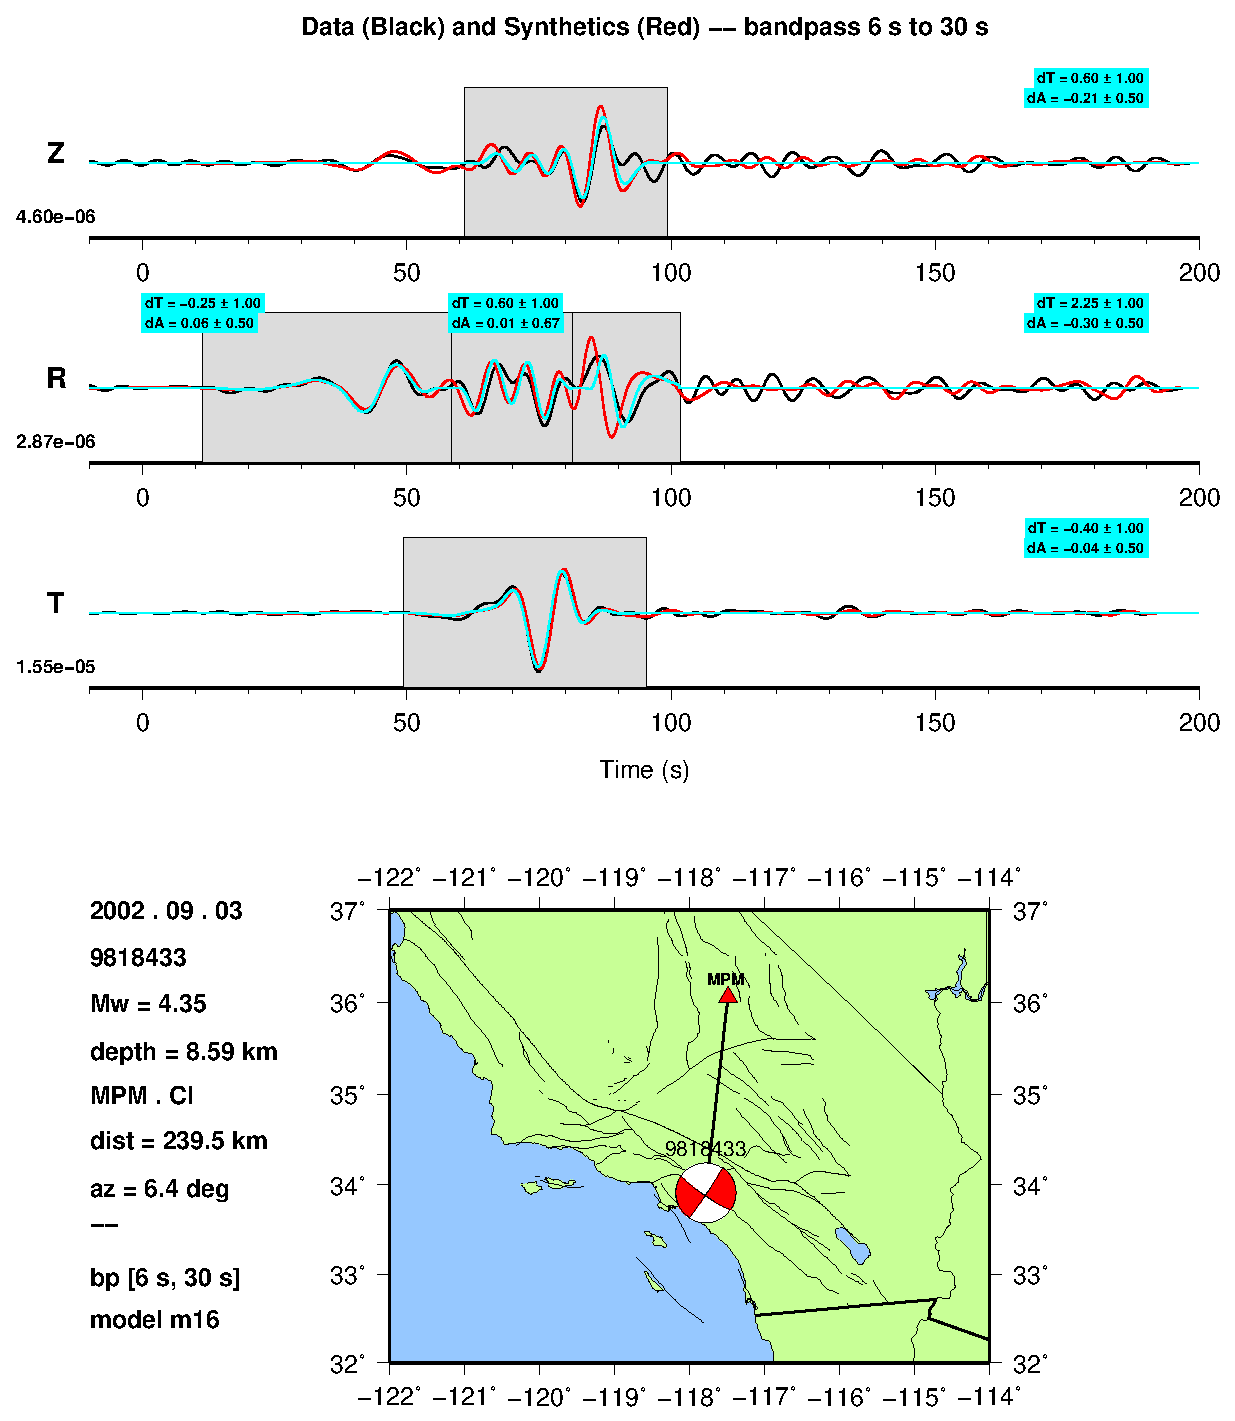
\includegraphics[width=17cm]{9818433_T006_T030_MPM_CI_m16_win.eps}
\caption[]
{{
Test case seismograms with {\tt COMPUTE$\_$ADJOINT$\_$SOURCE = .false.}.  Plot shows a three-component seismogram: Z = vertical, R = radial, T = transverse.  Black is the observed records, red is the synthetics, and blue is the reconstructed synthetics, made by applying the $\Delta T$ and $\Delta \ln A$ measurements within each window to the synthetics.  No adjoint sources are plotted.
\label{fig:noadj}
}}
\end{figure}

\begin{figure}
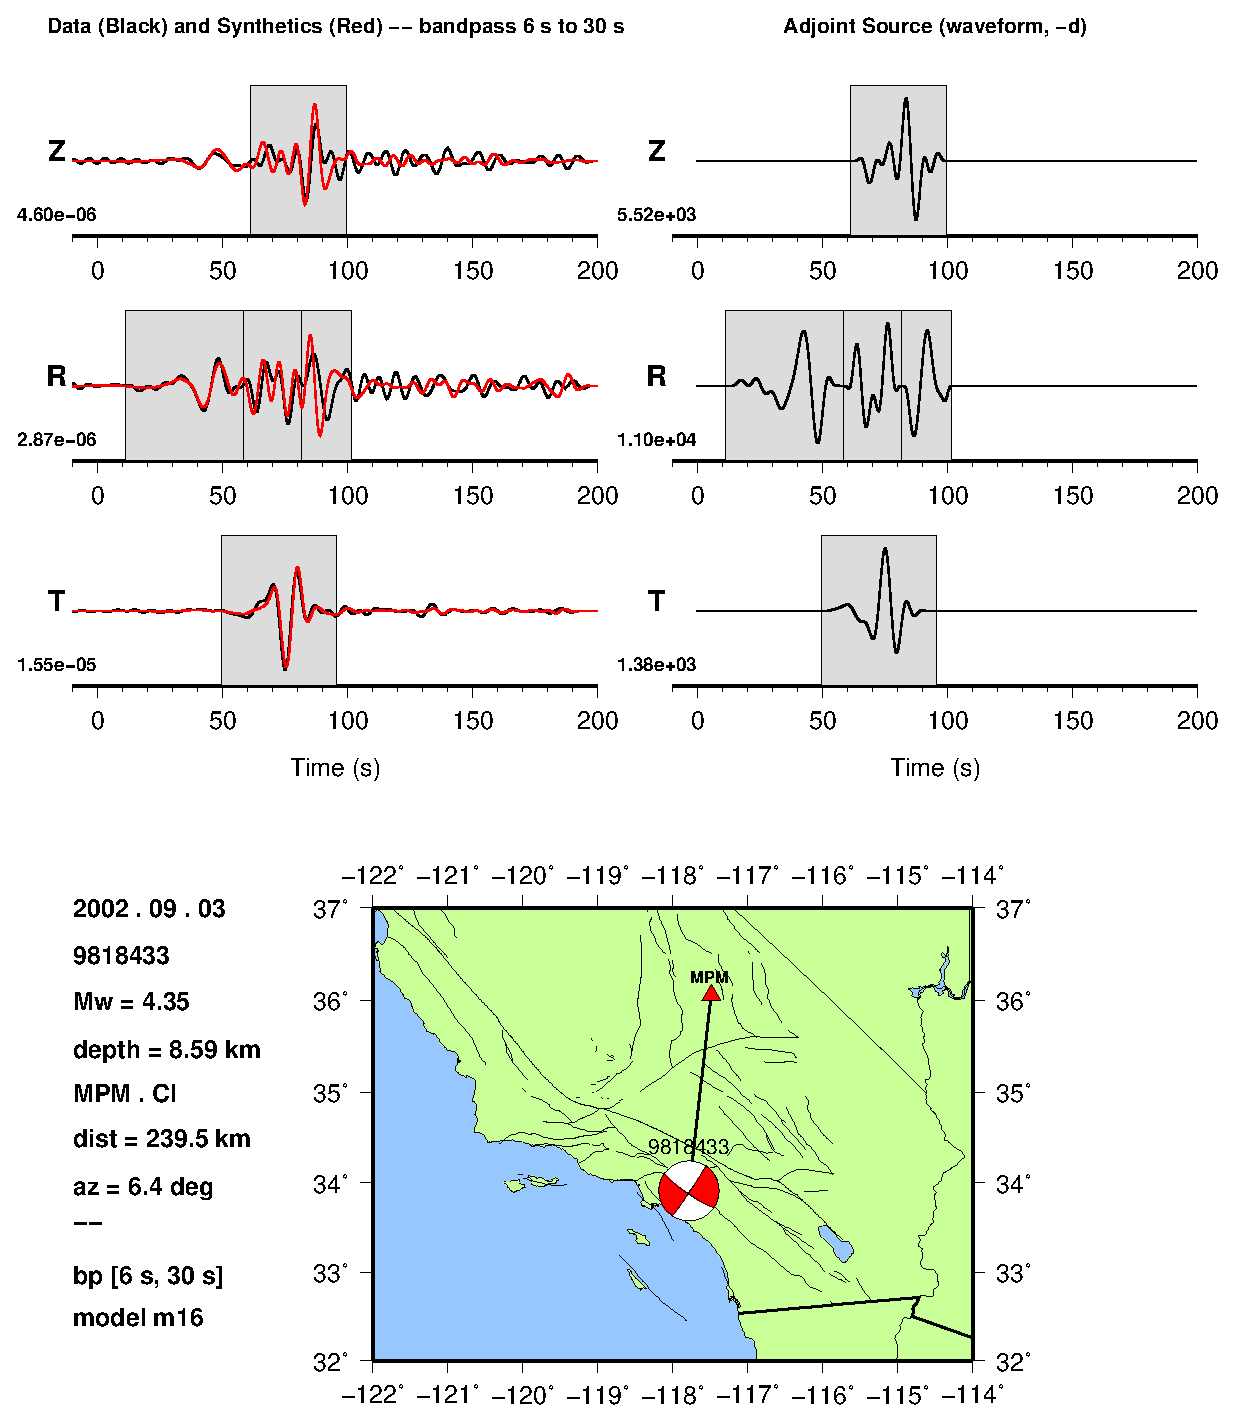
\includegraphics[width=17cm]{9818433_T006_T030_MPM_CI_m16_iker01_win_adj.eps}
\caption[]
{{
{\em Left:} Data (black), synthetics (red), and measurement windows.
{\em Right:} Adjoint sources constructed from the data alone ({\tt imeas = 1}), $-d(t)/\|d(t)\|^2$.
\label{fig:iker01}
}}
\end{figure}

\begin{figure}
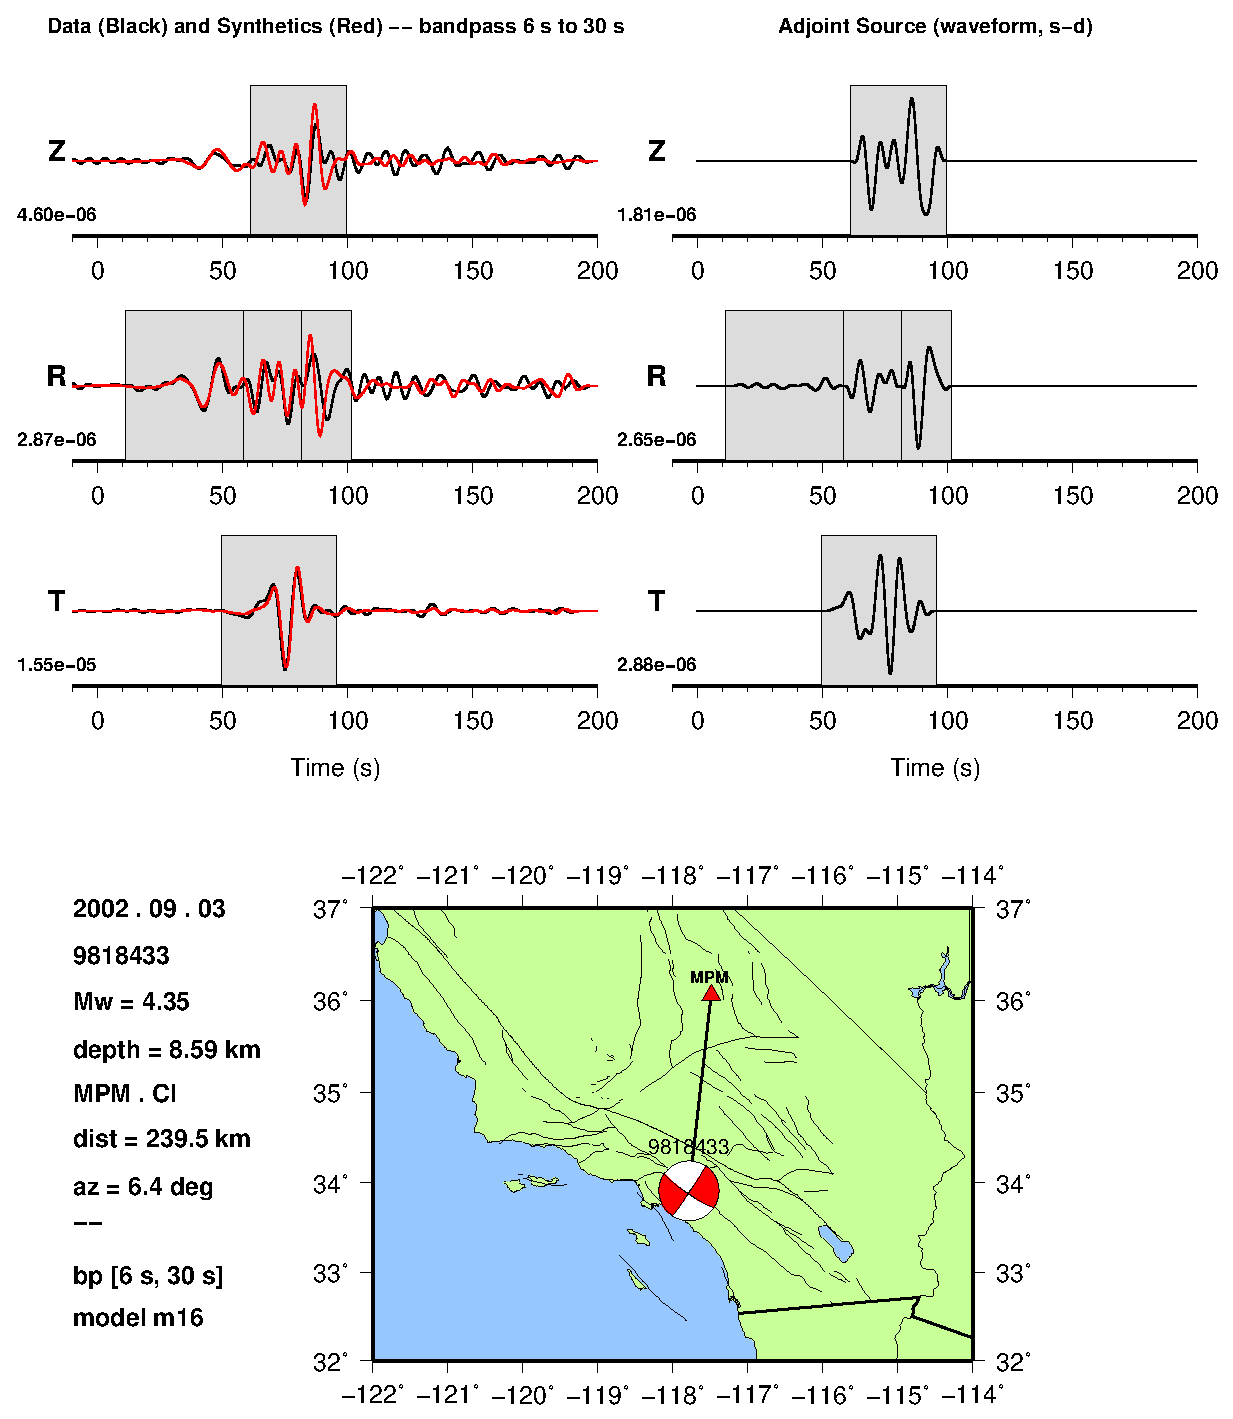
\includegraphics[width=17cm]{9818433_T006_T030_MPM_CI_m16_iker02_win_adj.eps}
\caption[]
{{
{\em Left:} Data (black), synthetics (red), and measurement windows.
{\em Right:} Adjoint sources for a waveform difference measurement ({\tt imeas = 2}), $\bs - \bd$.
\label{fig:iker02}
}}
\end{figure}

\begin{figure}
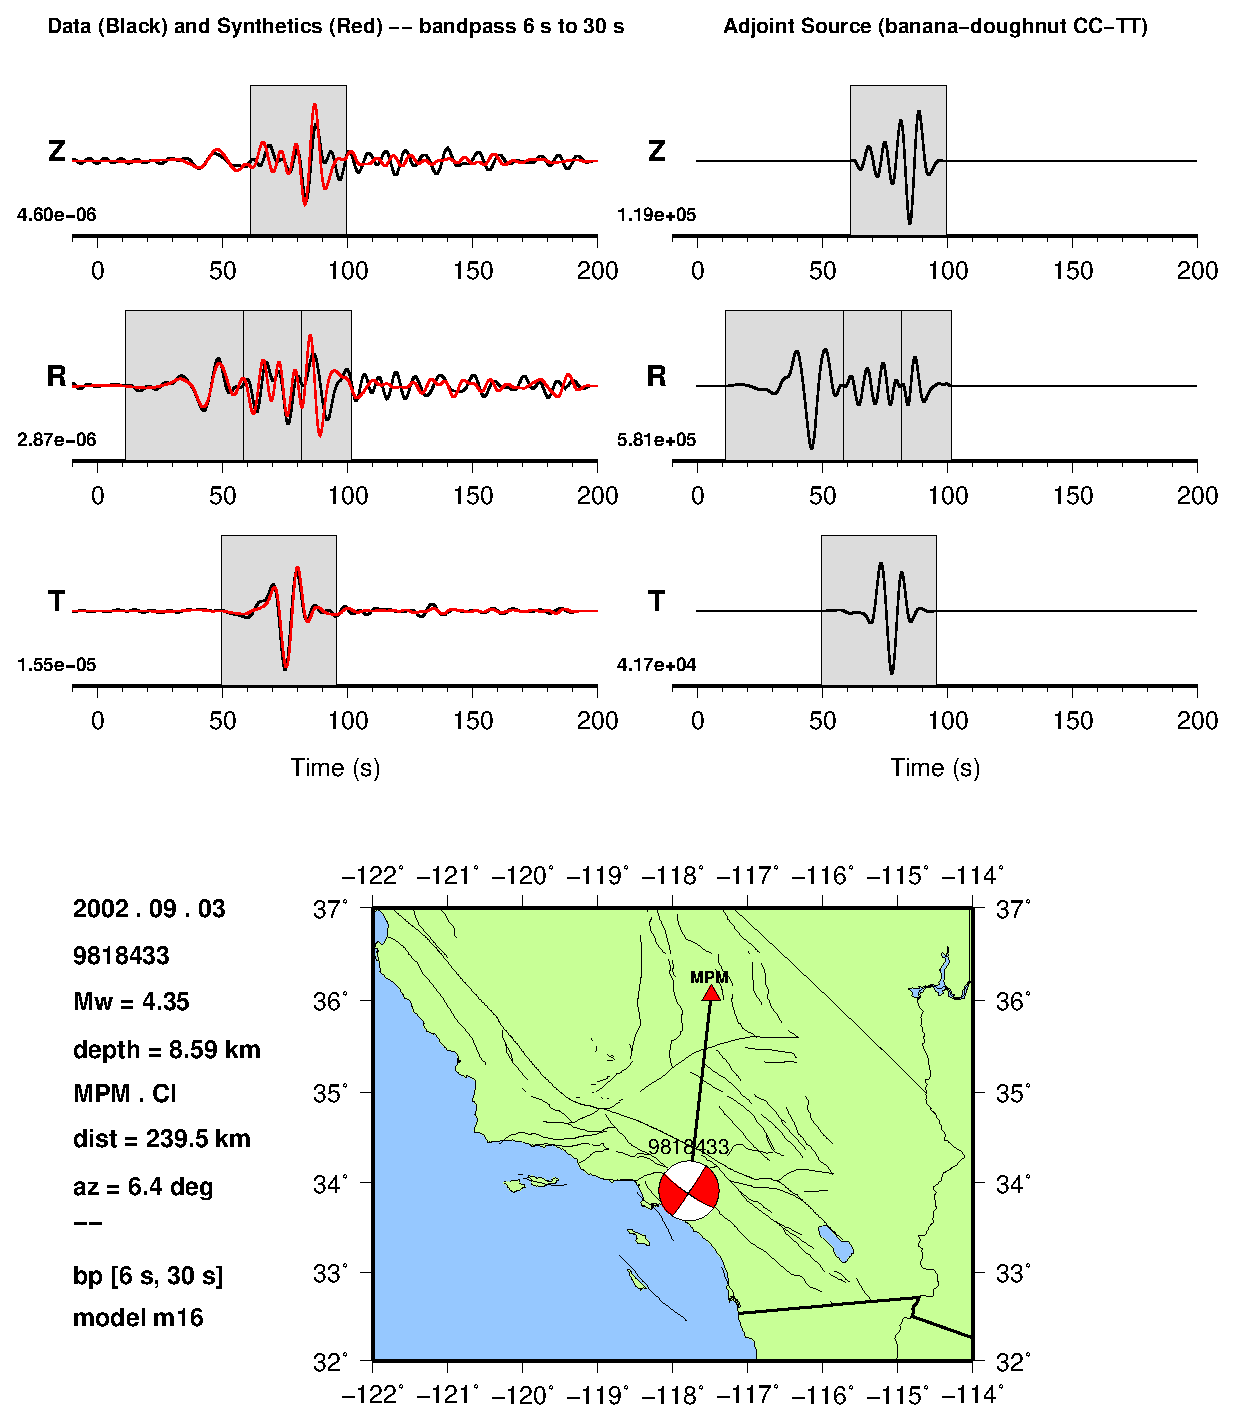
\includegraphics[width=17cm]{9818433_T006_T030_MPM_CI_m16_iker03_win_adj.eps}
\caption[]
{{
{\em Left:} Data (black), synthetics (red), and measurement windows.
{\em Right:} Adjoint sources for a sensitivity kernel based on a cross-correlation traveltime difference, $\Delta T$ ({\tt imeas = 3}).
\label{fig:iker03}
}}
\end{figure}


\begin{figure}
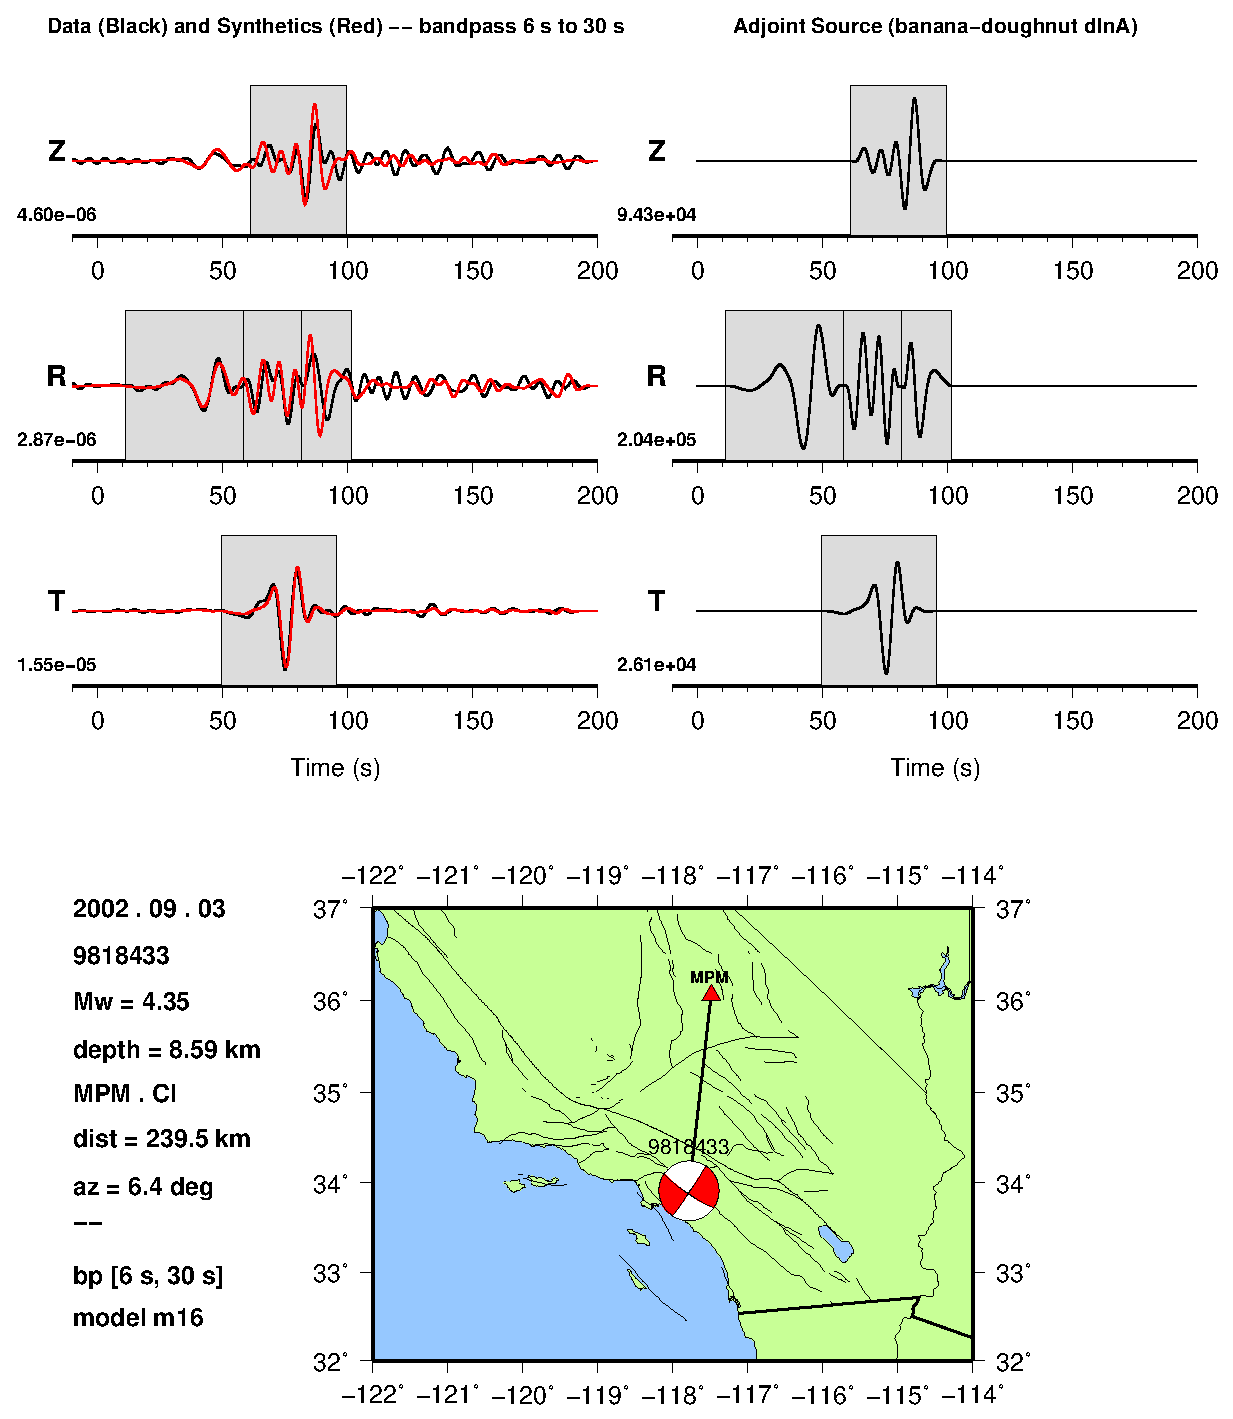
\includegraphics[width=17cm]{9818433_T006_T030_MPM_CI_m16_iker04_win_adj.eps}
\caption[]
{{
{\em Left:} Data (black), synthetics (red), and measurement windows.
{\em Right:} Adjoint sources for a sensitivity kernel based on an amplitude difference, $\Delta \ln A$ ({\tt imeas = 4}).
\label{fig:iker04}
}}
\end{figure}

\begin{figure}
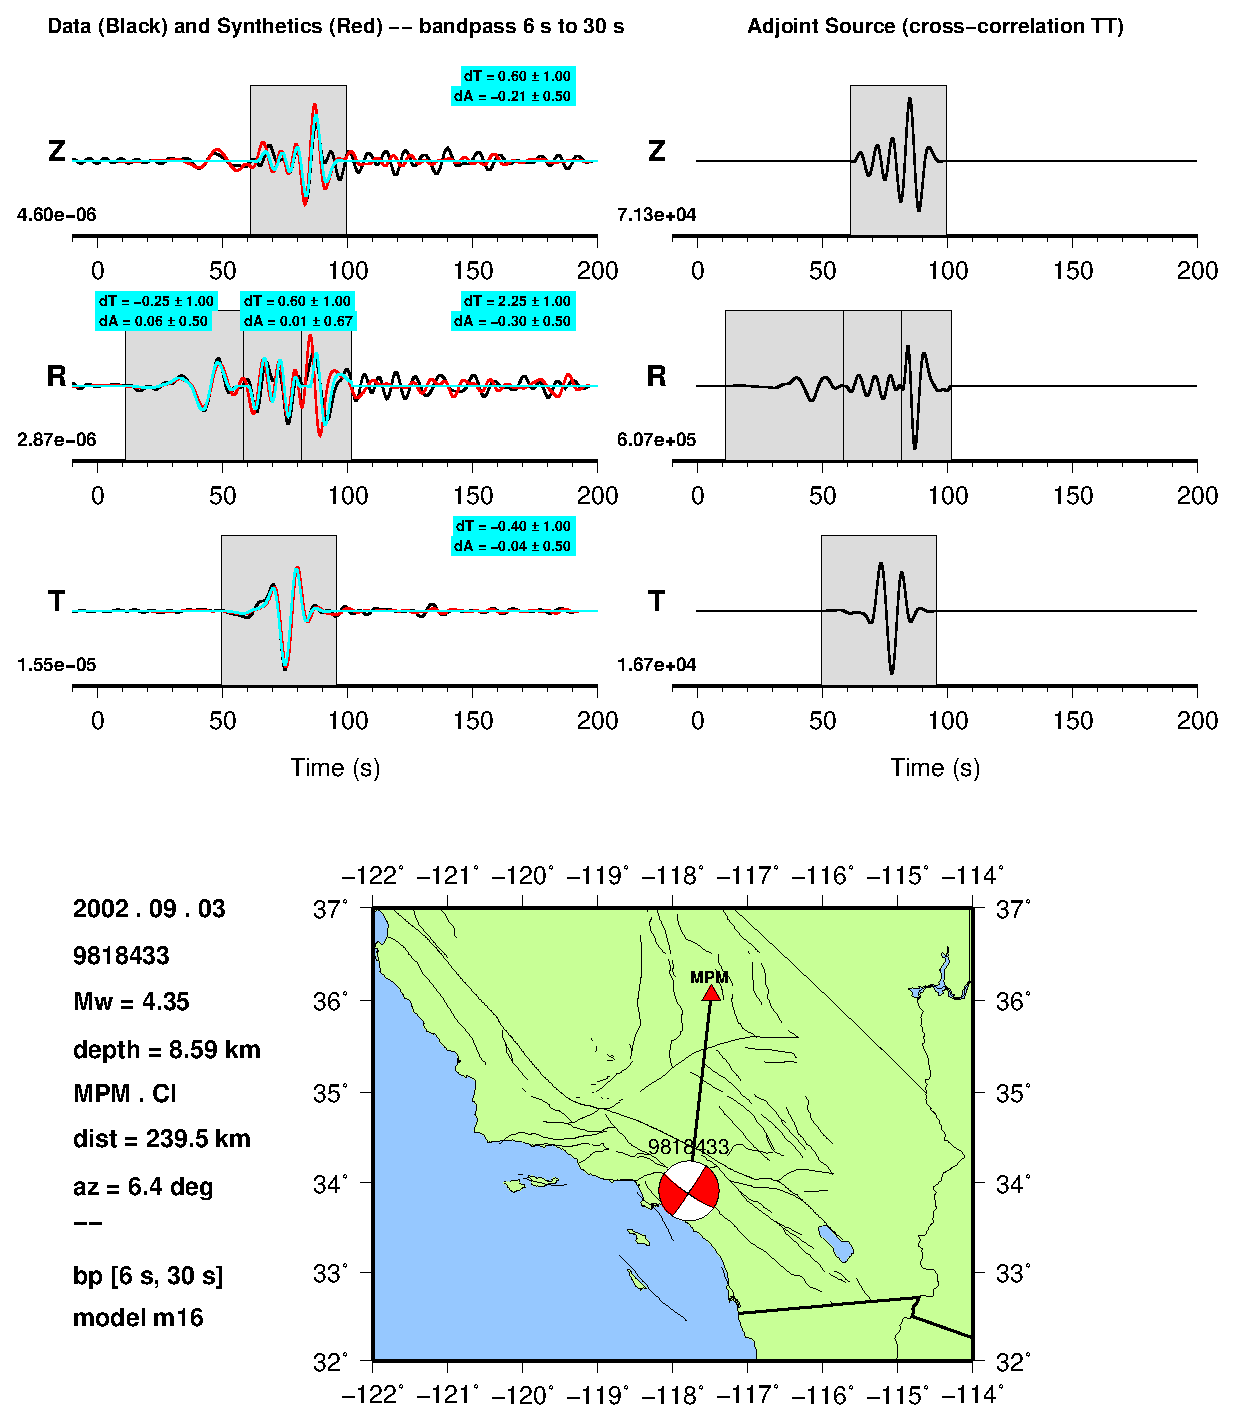
\includegraphics[width=17cm]{9818433_T006_T030_MPM_CI_m16_iker05_win_adj.eps}
\caption[]
{{
{\em Left:} Data (black), synthetics (red), and measurement windows.
{\em Right:} Adjoint sources for a cross-correlation traveltime difference, $\Delta T$ ({\tt imeas = 5}).
\label{fig:iker05}
}}
\end{figure}

\begin{figure}
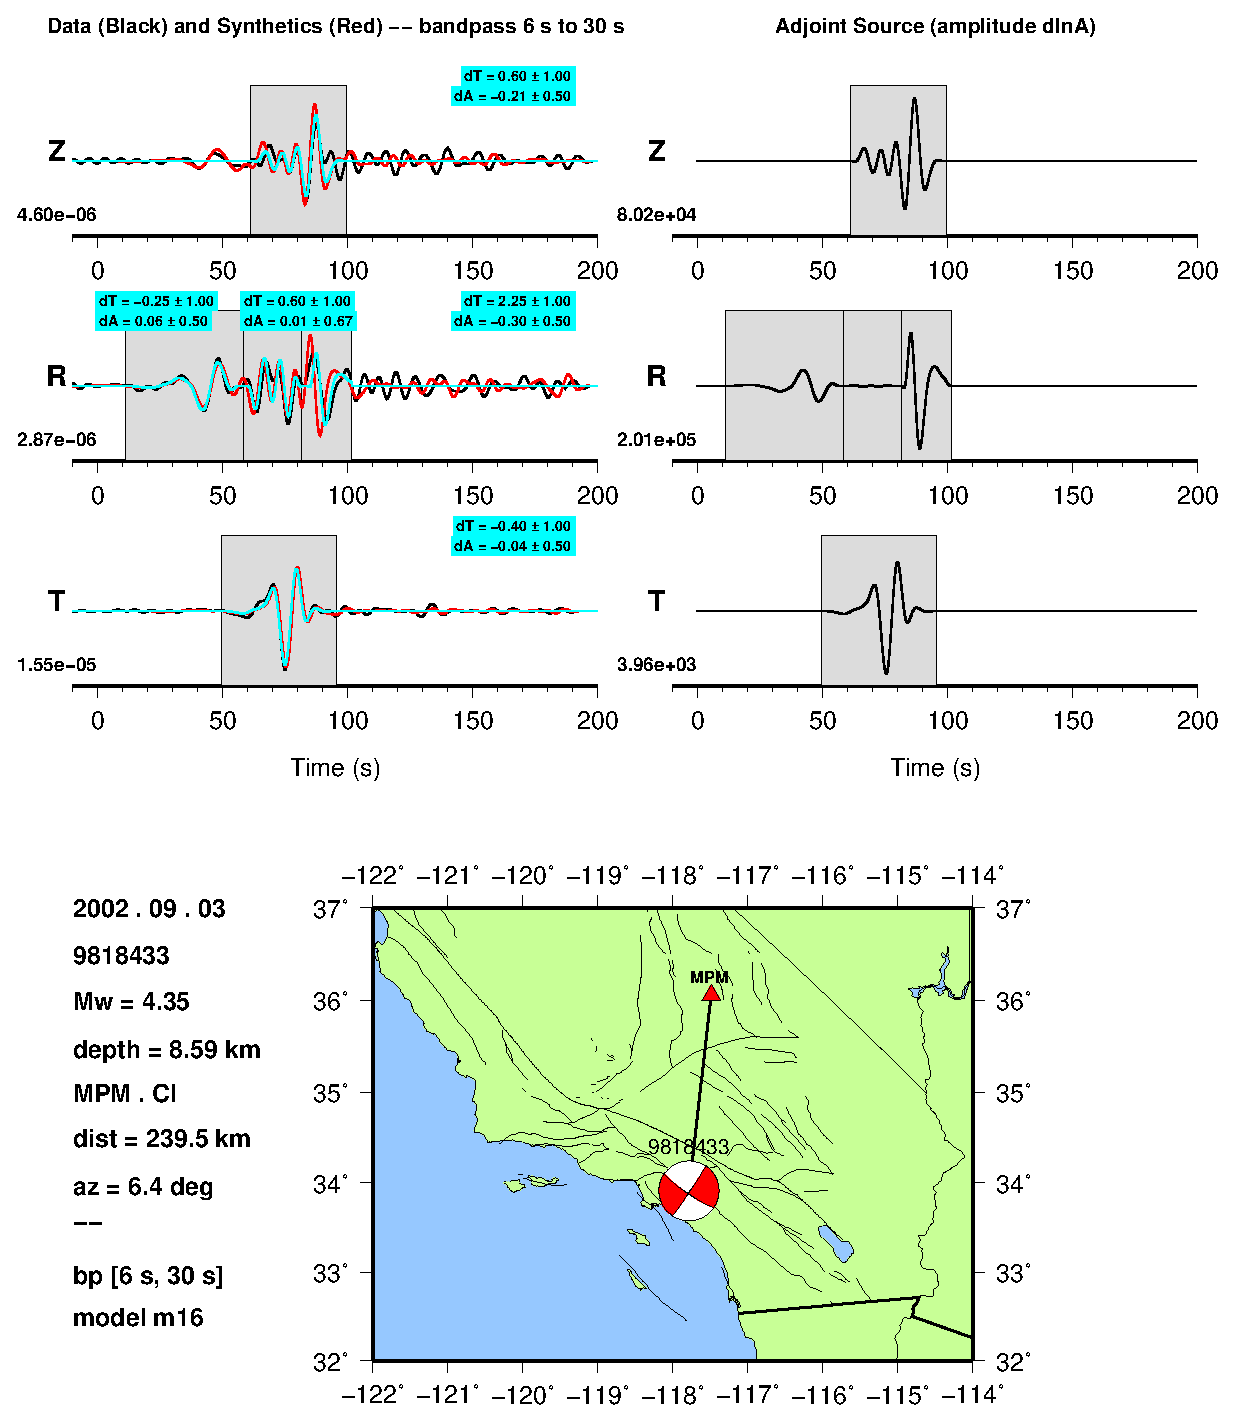
\includegraphics[width=17cm]{9818433_T006_T030_MPM_CI_m16_iker06_win_adj.eps}
\caption[]
{{
{\em Left:} Data (black), synthetics (red), and measurement windows.
{\em Right:} Adjoint sources for an amplitude difference, $\Delta \ln A$ ({\tt imeas = 6}).
\label{fig:iker06}
}}
\end{figure}

\begin{figure}
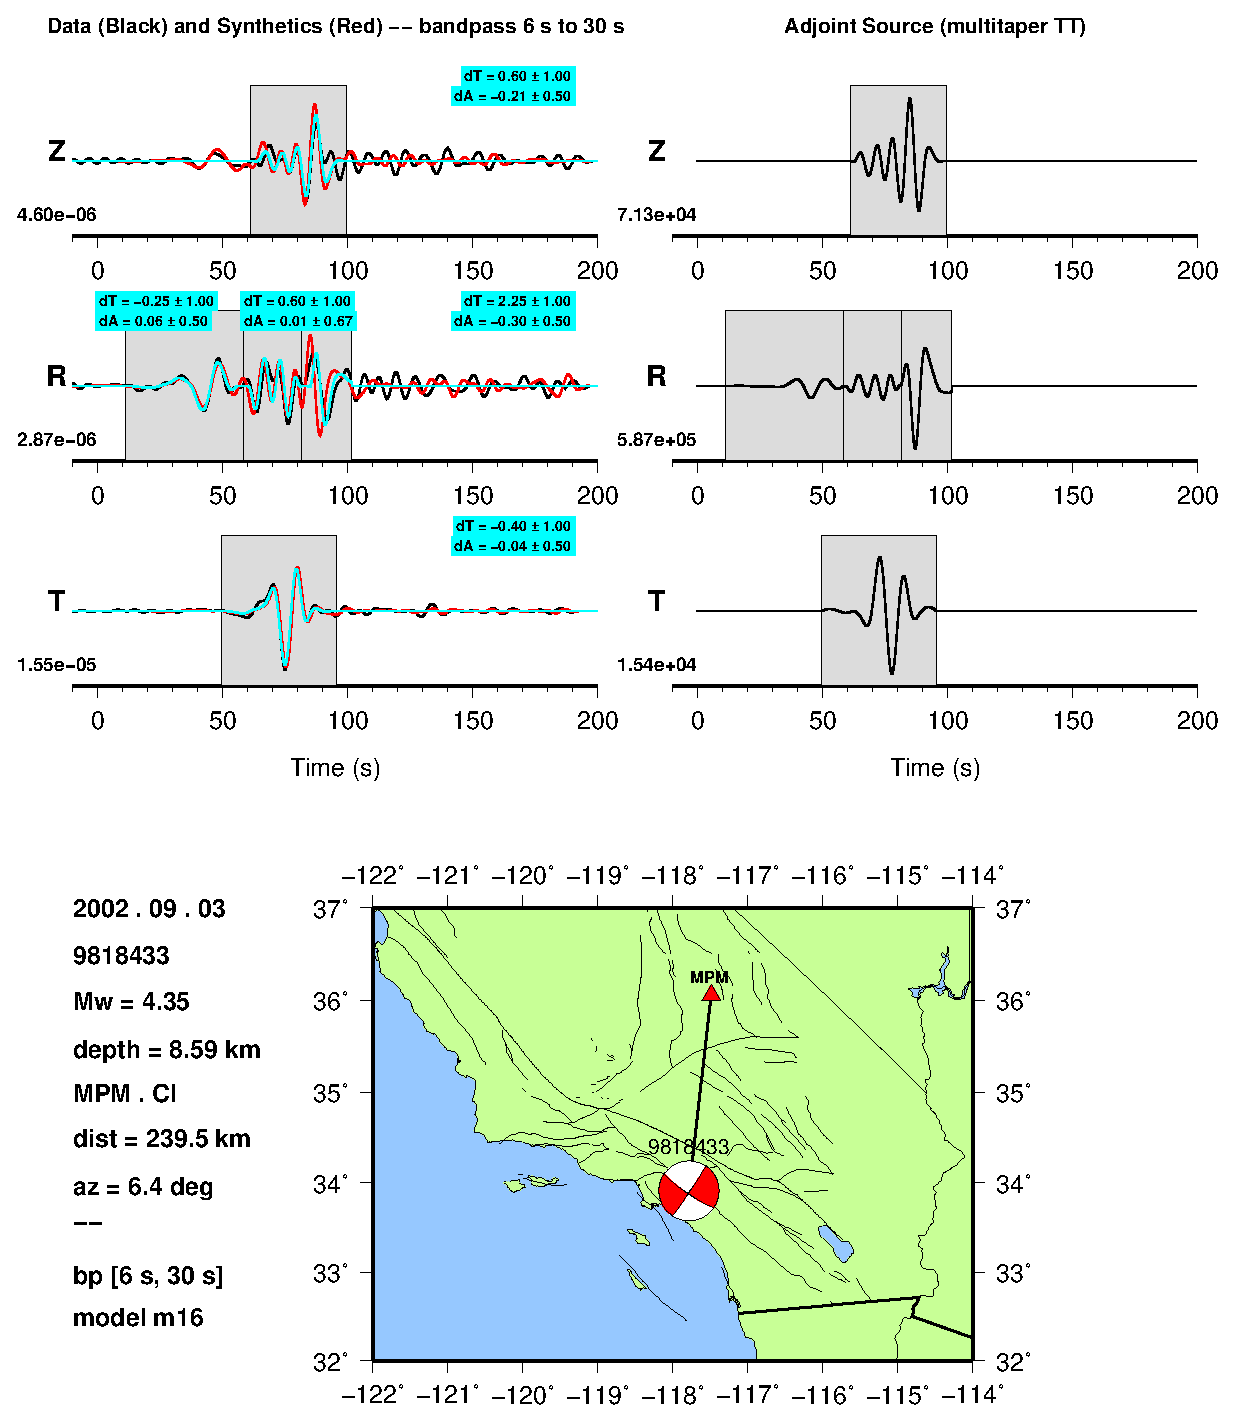
\includegraphics[width=17cm]{9818433_T006_T030_MPM_CI_m16_iker07_win_adj.eps}
\caption[]
{{
{\em Left:} Data (black), synthetics (red), and measurement windows.
{\em Right:} Adjoint sources for a multitaper traveltime difference ({\tt imeas = 7}).
\label{fig:iker07}
}}
\end{figure}

\begin{figure}
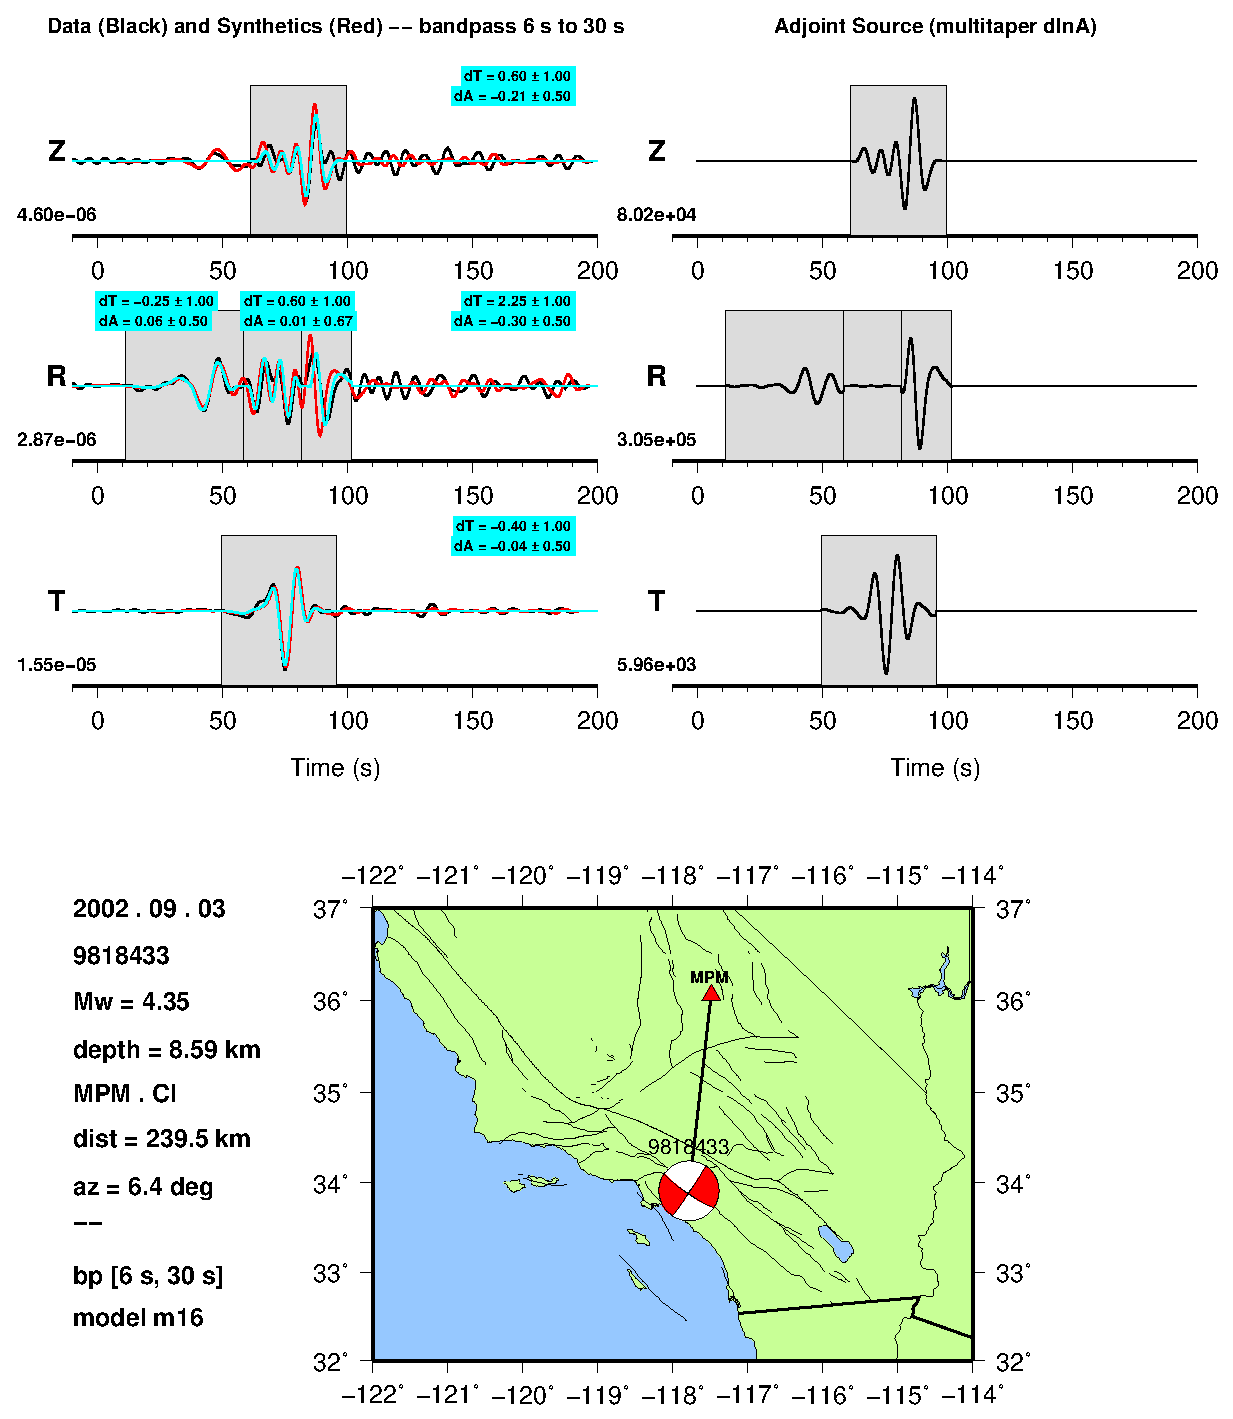
\includegraphics[width=17cm]{9818433_T006_T030_MPM_CI_m16_iker08_win_adj.eps}
\caption[]
{{
{\em Left:} Data (black), synthetics (red), and measurement windows.
{\em Right:} Adjoint sources for a multitaper amplitude difference ({\tt imeas = 8}).
\label{fig:iker08}
}}
\end{figure}

%-------------------------------------------------------------------
\end{document}
%-------------------------------------------------------------------
